%% An example of the article based on superfri.cls class file of
%% ``Supercomputing Frontiers and Innovations. An International Journal''
%% http://superfri.org/.

\documentclass{superfri}
\usepackage{graphicx}
\usepackage[hidelinks]{hyperref}
\usepackage{multirow}
\usepackage{caption}
\usepackage{subcaption}
\usepackage{adjustbox}
\usepackage{amssymb}
\usepackage{geometry}
\usepackage{pgfplots}
\usepackage{tikz}
\usepackage{float}
\usetikzlibrary{patterns}
\usepgfplotslibrary{groupplots}
\pgfplotsset{compat=1.9, every axis/.append style={
                    label style={font=\tiny},
                    tick label style={font=\tiny},
                    legend style={font=\tiny},
                    height=6cm
                    }}
\usepackage{pgfkeys}
    \newenvironment{customlegend}[1][]{%
        \begingroup
        \csname pgfplots@init@cleared@structures\endcsname
        \pgfplotsset{#1}%
    }{%
        \csname pgfplots@createlegend\endcsname
        \endgroup
    }%
    \def\addlegendimage{\csname pgfplots@addlegendimage\endcsname}

%%\captionsetup[subfigure]{labelformat=simple} % default is 'parens'
%%\captionsetup[subfigure]{width=0.9\textwidth}
%%\renewcommand\thesubfigure{\thefigure.\alph{subfigure}.}
\DeclareCaptionSubType*[alph]{figure}
\captionsetup[subfigure]{labelformat=simple,labelsep=period, width=0.9\textwidth}
% ------------
\bibliographystyle{superfri}

\begin{document}

\author{Damian Kaliszan, Norbert Meyer, Sebastian Petruczynik\footnote{\label{psnc}Poznan Supercomputing and Networking Center, ul. Jana Paw\l a II 10, 61-139 Pozna\'n, Poland}, Michael Gienger, Sergiy Gogolenko\footnote{\label{hlrs}High-Performance Computing Center Stuttgart, Nobelstra\ss{}e 19, 70569 Stuttgart, Germany}}

%%%\author{Alice~M.~Scientist\footnote{\label{susu}South Ural State University, Chelyabinsk, Russian Federation}$^{,2}$\orcidID{0000-1111-2222-3333} \and  Bob~A.~Scientist\footnoteref{susu} \and Derek~R.~Author\footnote{\label{msu}Lomonosov Moscow State University, Moscow, Russian Federation}\orcidID{1111-2222-3333-4444}


\title{HPC processors benchmarking assessment for Global System Science applications}
%%\thanks{The paper is recommended for publication by the Program Committee of the International Scientific Conference "Parallel computational technologies (PCT) 2018".}}

\maketitle{}
\begin{abstract}
\label{sec:abstract}
The work undertaken in this paper was done in the Centre of Excellence for Global Systems Science (CoeGSS), an interdisciplinary project, funded by the European Commission. The project provides decision-support in the face of global challenges (e.g. the network structure of the world economy, energy, water and food supply systems, the global financial system or the global city system, and the scientific community). It brings together HPC and global systems science. 
This paper presents a proposition of GSS benchmark with the aim to find the most suitable HPC architecture and the best HPC system which allows to run GSS applications effectively. 
The outcome of the analysis is defining a benchmark which represents the average GSS environment in a good way. Three exemplary challenges were defined as pilot applications: Health Habits, Green Growth and Global Urbanisation extended with additional applications from GSS ecosystem. They have been tested on a small set of new HPC platforms based on Intel Xeon Gold 6140, AMD Epyc, ARM Hi1616 and IBM Power8+ processors. 
Results of the tests provide the architecture comparison for different applications based on execution times, TDPs\footnote{Thermal Design Power} and TCO\footnote{Total Cost of Ownership} as the basic metrics used for providing a ranking of HPC architectures. Finally, the analysis or the results is thought to be valuable information for the GSS community for future purposes to determine their specific demands as well as - in general - to help develop a mature final benchmark set reflecting the GSS environment requirements and speciality.
\keywords{Global Systems Science, HPC benchmarks, parallel applications, 
e-Infrastructure evaluation}
\end{abstract}



% -----------------------------------------------------------------------

\section*{Introduction}
\label{sec:intro}
Global Systems Science (GSS) is a branch of science using specific knowledge and techniques to evaluate the impact of policies and people's relation on various global phenomena such as climate change, financial crises, pandemic spread, growth of the cities, human migration, etc. This document addresses the question ``which HPC architectures among the recently introduced are best to run GSS applications most effectively?''. Such aliases as ``the best'' or ``most effectively'' may obviously have different meanings for different people. While for some it may be the fastest execution time, others may be interested in the price-performance ratio calculated as the price of a processor multiplied by total execution time (for given architecture) or the least carbon footprint left, calculated as a product of TDP and total execution time.
For the purpose of this study, the authors acquired cutting-edge processors from four major vendors -- Intel, AMD, HiSilicon, and IBM. In particular, we benchmarked GSS applications on Intel\textregistered Xeon\textregistered Gold 6140 \cite{INTELXEONGOLD6140} 2-node cluster, AMD Epyc\textsuperscript{TM} 7551 single node, ARM Hi1616 2-node cluster, IBM Power8+ \cite{IBMPOWER8} single node, and -- as a reference testbed -- Eagle cluster located at Poznan Supercomputing and Networking Center (Poland) equipped with Intel\textregistered  Xeon\textregistered Haswell E5-2697 v3 processors.
The set of tested applications (called a \textit{GSS benchmark} here) covers many research areas from the entire GSS field.

The rest of the paper is organized as follows.
Section\,\ref{sec:benchmark} describes benchmark and the experimental setup.
More specifically, we introduce applications chosen for the benchmark and motivate this choice,
present technical overview of the testbeds where the tests were launched,
and discuss approach selected for measuring performance metrics.
In Section\,\ref{sec:analysis}, we shortly overview main benchmarking results.
In particular, we emphasize on the applicability of those results for the hardware/software co-design.
Section\,\ref{sec:summary} contains statements for the most relevant conclusions.
Finally, we end our paper with formulation of the directions for future research.


\section{Benchmark and experimental setup}
\label{sec:benchmark}
\subsection{Representative GSS applications selected for the benchmark}
Functionally, the  benchmarked  applications  can  be  categorized  into  two  groups: HPC-compliant social simulation software and large-scale CFD (Computational Fluid Dynamics) applications. From the perspective of programming languages, GSS benchmark covered applications written in C++ and Python, which are the most popular programming languages among GSS experts who use HPC.
% The applications have been selected both from projects provided by the project and generally available in public repositories.
This section contains a short description of tested applications: OpenSWPC, ABM4Py, CCTM, CM1, IPF, HWRF, Pandora/GG.

\subsubsection{HPC-compliant social simulation software}

\paragraph{ABM4Py} (ABMS for Python) is a distributed agent-based modelling and simulation framework for fast prototyping agent based components of GSS models \cite{2018:abm4py}.
Agent-based models implemented in \textsf{ABM4Py} follow the graph-based representation \cite{2018:abm4py,2017:graph_abms}.
Namely, agents and loci of interactions are interconnected into a complicated dynamic network, and agent-based simulation reflects possible temporal evolution of this network.

In order to benchmark this framework, we prepared a simple agent-based model within \textsf{ABM4Py} which implements random walk with simple interaction of agents.
This toy model allows to measure the most relevant performance metrics for \textsf{ABM4Py} including elapsed time, I/O, waiting time, and synchronization time.
In order to enable comparison of the \textsf{ABM4Py} framework with \textsf{Pandora} frameworks (see below), out toy model uses a 2D mesh as a topology of environment.
More specifically, we test against two cases -- one where layer shape size is set to 64x64 and the second with a size of 128x128.
% For both cases the possible numbers of MPI processes used were limited to square numbers (1,4,9,16...).

\iffalse
Two types of entities are created: location, as part of a spatial domain, and acting agents that follow some decision rule and interact with each other. The agents are distributed uniformly on a 2D area. The spatial proximity increases the likelihood of agents to get connected. Each agent has only one property "A", which is initiated as a random floating point number between 0 and 1 and is connected with other m agents.
At each step the agents perform the same action pattern. If the average of all values "A" of all connected agents is less than 0.5, the agents draw a new property "A" for themselves. It is to observe if the global average of "A" is affected by the decision rule and, if so, how.
This minimal example therefore contains a computational component per agent (action) and a communication component. The property "A" is synchronised via ghost agents between the processes.
Depending on whether the focus is on weak or strong scaling, the example setup can adapt to the number of used processes.
\fi

\underline{Project repository}: \url{https://github.com/CoeGSS-Project/abm4py}

\underline{Downloads}: \url{https://github.com/CoeGSS-Project/abm4py/archive/master.zip}

\iffalse
\underline{Use case description}

The application is purely python-based code that requires several modules among which the most important is \textit{h5py} (pythonic interface to the HDF5 binary data format). It additionally requires \textit{class\_auxiliary.pyc,  class\_graph.pyc} and \textit{lib\_gcfabm.pyc} files containing the application's byte code. Additionally, the python environment has to be equipped with additional modules preinstalled such as \textit{numpy, mpi4py, matplotlib, pandas}, etc.
\fi

\paragraph{Pandora/GG} application serves for benchmarking \textsf{Pandora} agent-based modelling and simulation framework.
In contrast to \textsf{ABM4Py}, \textsf{Pandora} supports only raster inputs
which restricts this framework to agent-based models with 2D mesh as a topology of environment.
On the other hand, \textsf{Pandora} is implemented in C++,
which allows to reach higher performance compared to Python-based \textsf{ABM4Py} framework.

Our Pandora/GG application implements the green growth agent-based model, first proposed in \cite{2017:gg_pilot}, within \textsf{Pandora} framework.
%Green Growth using Pandora library
The green growth model is an innovation-diffusion model for electric cars with a global scope and a fine-scale spatial data resolution.
%% The model is agent-based and is studying the car-centered global system in view of a green growth transition.

\iffalse
There are two implementations of his model: deterministic and a stochastic whose implementation for benchmarking purposes was used \cite{2018:abm4py}.
In this preliminary version of the green growth pilot, authors consider only two classes of cars: "green" cars, which for now correspond to battery electric vehicles due to data availability, and "brown" ones. Cars are distributed on a gridded global map, that is, in the first instance "agents" are simply cells in the grid, which automatically specifies a neighbourhood network between them, and their characteristics are a number of brown and one of green cars. Each cell at each time step computes the number of new cars to be added from the total numbers exogenous given and a percentage of cars being scrapped.
\fi

\underline{Project Web-page}: \url{http://xrubio.github.io/pandora/}

\underline{Downloads}: \url{https://github.com/xrubio/pandora/tarball/master}
\iffalse
\underline{Use case description}

The first step was to compile the library itself using SCons \cite{SCONS} as the main building tool.  It is open-source, python-based and next generation substitution of make utility. Version 2.4.1 of the tool  was used because the newest version was not compatible with the build input file (/textit{SConstruct}). For the build process Pandora \cite{2014:pandora} requires three additional, external libraries: \textit{HDF5, GDAL} and \textit{BOOST}. In the case of GDAL, version 1.11.5 was used for similar reasons to SCons. GDAL is a Geospatial Data Abstraction Library and presents a single raster abstract data model and single vector abstract data model to the calling application for all supported formats. It also comes with a variety of useful command line utilities for data translation and processing. Finally, Pandora installation required a BOOST C++ library built in place.
Depending on the hardware and system capabilities the following MPI libraries were used: Intel\textregistered MPI Library for Linux* OS, Version 2017 Update 1, Open MPI 1.10.2 (ARM), impi 5.0.3.048 (Eagle).
Input data for benchmark has been delivered as two maps (Europe and world) with two different resolutions 840x680 and 8640x3432. 

The above applications were cross-tested with selected processor architectures. The only exception is HWRF (Hurricane WRF), which could not be compiled on the ARM and Power8+ architectures due to the scale of this application and the difficulty in the compilation process.
Each test has been repeated twice with the measurements for minimum wall time selected to be reported. It is worth noticing that some results reveal unusual and difficult-to-explain behavior in memory consumption and/or I/O, which cannot be anticipated based on processor architecture or node configuration. These cases are supposed to be a subject of future analysis by applications authors or GSS community.
In general, the characteristic of the applications is found to be different and varying from I/O dependent to purely computational.
\fi

\paragraph{IPF} (iterative proportional fitting) is a "technique that can be used to adjust a distribution reported in one data set by totals reported in others. IPF is used to revise tables of data where the information is incomplete, inaccurate, outdated, or a sample" \cite{1912:ipf}.
This procedure reconstructs a contingency matrix based on the known marginals in an unbiased way.
Nowadays, IPF and its derivatives (e.g., IPU) constitute the computational core of the most popular techniques for gerenating synthetic data which serve as input for agent-based socail simulations \cite{2017:synpop}.

Despite its popularity, we are not aware of any HPC-compliant open-source implementation of IPF.
In order to overcome this obstacle,
we coded a simple IPF process using linear algebra kernels from \textsf{ScaLAPACK}.
This simple implementation was a baseline for our IPF benchmark.

\iffalse
IPF can be applied to multidimensional matrices, but the multidimensional case is a simple generalization of the two-dimensional case on which we base our presentation.
IPF fits the matrix coefficients so that the sums of elements of every row and every column are equal to the given respective marginals. The initial contingency matrix values are either all, or are based on some known correlation data (such as a micro sample). In general, IPF solves an underspecified problem, and its result is the maximum likelihood estimation assuming that the elements of the matrix are drawn from the Poisson distribution given by the initial contingency matrix.

IPF is often performed to fit a contingency matrix to known marginals as one step of synthetic population generation. If a lower-dimension contingency matrix is known, their values can be used as marginal for IPF, which then performs fitting that matches the correlations defined by this contingency matrix \cite{2018:norman}.
The IPF procedure is often followed by sampling, which uses the values from the reconstructed contingency matrix as weights. It may also be followed by the Iterative Proportional Updating (IPU) procedure, which uses reconstructed contingency matrices for individuals and households, and a micro sample of households containing individuals to perform individual-household assignment.

\underline{Use case description}

The benchmarked IPF implementation performs the IPF procedure for a 2-dimensional matrix.
The implementation is written in C programming language and uses the MPI and PBLAS APIs. MPI and PBLAS are common HPC APIs whose implementations are available on many platforms. On a typical Linux systems they can be provided by the OpenMPI, OpenBLAS and \textsf{ScaLAPACK} open-source packages. On HPC systems they are typically provided by proprietary libraries, such as the Cray MPI library, the Cray libsci library or the Intel MKL library.
The implementation uses MPI to launch computing processes on different computational nodes, and perform message-based communication between them. The PBLAS API which, if built on top of MPI, provides operations on distributed vectors and matrices, such as computing a sum of a distributed vector (pdasum) or scaling a distributed vector (pdscal), both of which are used by the implementation.
The PBLAS operations assume that the distributed vectors and matrices are laid out according to the one- or two-dimensional block-cyclic distribution. The distribution is parametrised by the block size, which affects the performance of the operations performed on the vectors and matrices.
The implementation performs iterations until the maximum-norm error between the target marginals and the marginal computed from the matrix falls below a threshold value.

For testing purposes IPF was compiled against \textsf{ScaLAPACK} and OpenBLAS. 
Application parameters \textit{PROCROWS, PROCCOLS, ROWBLOCK} and \textit{COLBLOCK}  and a limited number of MPI processes to \textit{PROCROWS* PROCCOLS}. \textit{ROWBLOCK} and \textit{COLBLOCK} are required to be set independently with values equal to the power of 2.

\fi

\textit{Note}: These IPF codes are not published with open access on the Internet yet.

\subsubsection{Large-scale CFD applications}

\paragraph{OpenSWPC} (Open-source Seismic Wave Propagation Code) is an open-source software fro large-scale simulation of seismic waves propagation (2D or 3D) by solving motion equations using the finite difference method (FDM) \cite{OpenSWPC2}. OpenSWPC is widely used in seismology. It ports easily and delivers good performance on different distributed systems varying from small PC clusters to large-scale supercomputers.
\iffalse
Without modifying the code, users can simulate seismic wave propagation using their own speed structure models and the necessary source representations in the input parameter file. The software code is equipped with a frequency-independent damping model based on a generalised Zener (standard linear solid - SLS model) body and an efficiently selected, perfectly matched boundary absorbing layer. It has different modes for the different input data types of the velocity structure model and different source representations, such as single force, torque tensioner and flat frequency, which can be easily selected by input parameters. Common binary data formats, a common network data form (NetCDF), and a seismic analysis code (SAC) are used to input a heterogeneous structure model and simulation results so that users can easily operate their input and output data sets. All codes are written in Fortran 2003 and are available with detailed documents in a public repository.
\fi

\underline{Project repository}: \url{https://github.com/takuto-maeda/OpenSWPC}

\underline{Downloads}: \url{https://github.com/takuto-maeda/OpenSWPC/releases}
\iffalse
\underline{Use case description}

The first step was to install the required system packages such as \textit{gmt, gmt-dcw, gmt-gshhg, libnetcdf-dev}. The next one required to run \textit{gen\_JIVSM.sh} script to generate files used as a model input around Japanese Islands for seismic wave propagation in and around Japan. They describe 3D complicated subsurface structures of the earth. The above script used the following input files \textit{lp2012nankai-e\_str.zip, lp2012nankai-w\_str.zip} available from public repository at \cite{HERP} and \textit{ETOPO1\_Bed\_g\_gmt4.grd.gz} from \cite{NOAA} to be installed in the \textit{dataset/vmodel} folder.
Finally, inside the \textit{OpenSWPC/src} folder the files \textit{shared/makefile.arch} and \textit{shared/makefile-tools.arch} needed to be updated to fix the system paths.
After successful compilation an input file (e.g example/input.inf) had to be provided to run the application. Critical attributes influencing the run times included the grid size defined by \textit{nx = 1000, ny = 875, nz = 200}   (total grid number in x, y and z directions) and \textit{nt = 100}  (time step number)

Depending on the hardware and installed libraries the following MPI versions were used: Intel\textregistered MPI Library for Linux\textregistered OS, Version 2017 2017.1.132 (2-node Intel\textregistered\ Xeon\textregistered\ Gold 6140, Eagle cluster), Open MPI 1.10.2 (ARM, AMD Epyc\textsuperscript{TM})
\fi



\paragraph{CMAQ/CCTM}
(Community Air Multiscale Quality Modelling System) is an active open-source project of the U.S. EPA (\textit{Environmental Protection Agency}) %Computational Exposure Division
that delivers a suite of programs for conducting air quality model simulations. %CMAQ is supported by the CMAS Center.
%% It combines current knowledge in atmospheric science and air quality modelling with multi-processor computing techniques %% in an open-source framework
%% to deliver fast, technically sound estimates of ozone, particulates, toxins, and acid deposition.
CCTM (\textit{The CMAQ Chemistry-Transport Mode}) is a parallel implementation of the advanced chemical transport model in CMAQ
which is often used in computer-aided policy making for improving air quality \cite{CHEMEL2014410}.
It is the only CMAQ program that can be run in parallel.

CCTM runs require large input datasets with complicated file structure.
In our study, we used the official single day simulation benchmark dataset distributed by EPA \cite{EPA}.

\underline{Project Web-page}: \url{https://www.cmascenter.org/cmaq}

\underline{Downloads}: \url{https://www.cmascenter.org/download/forms/step_2.cfm?prod=2}

\iffalse
\underline{Use case description}

The following libraries have to be installed prior to building CCTM: \textit{NetCDF, NetCDF Fortran, IOAPI}. When installed, the following scripts could have been initiated to finish the installation and run the application itself: \textit{config\_cmaq.csh, bldit\_project.csh, bldit\_cctm.csh, run\_cct.csh}.
Benchmark data have been downloaded based on the information provided by EPA for a single day \cite{EPA}.
\fi

\paragraph{CM1} is a three-dimensional, time-dependent, non-hydrostatic numerical model. %that has been developed primarily by George Bryan at The Pennsylvania State University (PSU) (circa 2000-2002) and at the National Center for Atmospheric Research (NCAR) (2003-present).
CM1 is designed primarily for idealized research, particularly for deep precipitating convection and for studies of relatively small-scale processes in the Earth's atmosphere, such as thunderstorms \cite{CM1}.

\iffalse
CM1 is also designed for distributed-memory computing systems. In CM1 there are three models of parallelization. Shared memory parallelization with OpenMP, distributed memory using MPI and mix of both of them - hybrid OpenMP/MPI.
\fi

\underline{Project Web-page}: \url{http://www2.mmm.ucar.edu/people/bryan/cm1}

\underline{Downloads}: \url{https://github.com/NCAR/CM1}

\iffalse
\underline{Use case description}

CM1 use case contains the following steps: CM1 software download and unpack  \cite{CM1DATA}, compilation and build. When successfully compiled, a \textit{cm1.exe} binary file is created under \textit{cm1r19/run} directory. \textit{cm1r19/ run/ namelist.input} configuration file was used with appropriate \textit{nodex, nodey} and \textit{ppnode} values to let the simulation start on the given number of processors (NP). The simulation is started by calling mpirun: \textit{mpirun -np \$NP ./cm1.exe}
\fi

\paragraph{WRF} (Weather Research and Forecasting model) is an example of a well-scalable application,
which motivated us to add it to the set of tests in order to increase the variety of requirements of the {GSS benchmark}. 
%% Hurricane Katrina formed as Tropical Depression Twelve over the southeastern Bahamas on August 23, 2005, as the result of an interaction of a tropical wave and the remains of Tropical Depression Ten.
%% It strengthened into Tropical Storm Katrina on the morning of August 24 and continued to change its form and intensification on the following days and caused a lot of damage.
The Hurricane Weather Research and Forecasting (HWRF) model is a specialized version of the WRF model \cite{2018:hwrf}.
It is used to forecast the track and intensity of tropical cyclones.
% The HWRF modeling system, based on the NMM (non-hydrostatic mesoscale model) core of the WRF (Weather Research and Forecasting) model, is a high resolution coupled air-sea-land prediction model with a movable nested grid and with the applicability to the prediction problems of hurricane track, intensity, structure, and rainfall. The model uses a two-way interactive movable nested grid that follows the forecasted path of the tropical cyclone.

\underline{Project Web-page}: \url{https://dtcenter.org/HurrWRF/users}

\underline{Downloads}: \url{http://www.dtcenter.org/HurrWRF/users/downloads/index.php}

\iffalse
\underline{Hurricane WRF software}

% The model was developed by the National Oceanic and Atmospheric Administration (NOAA), the U.S. Naval Research Laboratory, the University of Rhode Island, and Florida State University. 
\fi


This document does not go further into theory as it is beyond its main subject.
We refer the interested reader for more technical details to the reports \cite{2017:coegss_benchmark1,2018:coegss_benchmark2}.

%%\input{description_tests}
\subsection{Configuration of testbeds used for the benchmark}
\label{sec:arch}
           
We executed our benchmark on four testbeds using cutting-edge processors recently introduced by four major processor vendors:
Xeon\textregistered Gold 6140 from Intel \cite{INTELXEONGOLD6140},
AMD Epyc\textsuperscript{TM} 7551 from AMD \cite{2019:epyc, now:epyc},
ARM Hi1616 from HiSilicon \cite{2017:hi1616,2019:hi1616},
and Power8 from IBM \cite{2015:power8,2016:power8}.
While
table~\ref{tab:clusterconfig} summarizes relevant technical characteristics of our testbeds,
the text below describes important architectural improvements introduced into the processors.

%https://en.wikichip.org/wiki/intel/xeon_gold/6140
%https://en.wikichip.org/wiki/amd/epyc/7551
%https://en.wikichip.org/wiki/hi1616
\begin{table}
\caption{Testbed characteristics}
\label{tab:clusterconfig}
\begin{adjustbox}{width=1\textwidth}
\small
\begin{tabular}{l|c|c|c|c|}
\cline{2-5}
\multicolumn{1}{c|}{} & \textbf{Intel\textregistered\ Xeon\textregistered\ Gold 6140} & \textbf{AMD Epyc\textsuperscript{TM} 7551} & \textbf{ARM Hi1616} & \textbf{Power8+ S822LC} \\ \hline
\multicolumn{1}{|l|}{\textbf{No. of nodes}} & 2 & 1 & 2 & 1 \\ \hline
\multicolumn{1}{|l|}{\textbf{Cores per node}} & 36 & 64 & 64 & 20 \\ \hline
\multicolumn{1}{|l|}{\textbf{CPU Frequency [GHz]}} & 2.3 & 2 & 2.4 & 2.92 \\ \hline
\multicolumn{1}{|l|}{\textbf{L1 (data) cache}} & 576 kB &  1 MB & 1 MB & 64 kB, 8-way \\ \hline
\multicolumn{1}{|l|}{\textbf{L2 cache}} & 18 MB & 16MB & 8MB & 512 kB, 8-way \\ \hline
\multicolumn{1}{|l|}{\textbf{L3 cache}} & 24.75 MB & 64 MB & 32 MB & 8 MB/core, 8-way \\ \hline
\multicolumn{1}{|l|}{\textbf{Mem type (channels)}} & DDR4-2666 (6) & DDR4-2400 (8) & DDR4-2400 (4) & ??? (4) \\ \hline
\multicolumn{1}{|l|}{\textbf{RAM [GB]}} & 192 & 512 & 128 & 512 \\ \hline
\multicolumn{1}{|l|}{\textbf{TDP [W]}} & 140 & 180 & 70 & 190 \\ \hline
\multicolumn{1}{|l|}{\textbf{Processor price [USD]}} & 2450 & 3743 & 300 & 1500 \\ \hline
\multicolumn{1}{|l|}{\textbf{Interconnect desc.}} & 10Gb Ethernet & 10Gb Ethernet & 10Gb Ethernet & 10Gb Ethernet \\ \hline
\multicolumn{1}{|l|}{\textbf{I/O and disks}} & SSD & SSD & SSD & SSD \\ \hline
\multicolumn{1}{|l|}{\textbf{OS version}} & Ubuntu 16.04.03 LTS & \multicolumn{1}{c|}{CentOS 6.9} & \multicolumn{1}{c|}{\begin{tabular}[c]{@{}l@{}}EulerOS release 2.0 (SP2),\\ Ubuntu 16.04.3 LTS\end{tabular}} & \multicolumn{1}{c|}{Ubuntu 16.04.2 LTS} \\ \hline
\multicolumn{5}{|c|}{Total bandwidth estimates (per node) [GBps]}  \\ \hline
\multicolumn{1}{|l|}{\textbf{L1 (data) cache}} & 3974 & 6144 & 7372 & 2803 \\ \hline
\multicolumn{1}{|l|}{\textbf{L2 cache}} & 3974 & 6144 & 7372 & 2803 \\ \hline
\multicolumn{1}{|l|}{\textbf{L3 cache}} & 5298 & 8192 & 9830 & 3738 \\ \hline
\multicolumn{1}{|l|}{\textbf{Total memory}} & 119.21 & 158.95 & 71.53 & 230 \\ \hline
\multicolumn{1}{|l|}{\textbf{SMP interconnect}} &  &  &  & 38.4 \\ \hline
\multicolumn{1}{|l|}{\textbf{PCIe interconnect}} & 192 & 256 & 184 & 128 \\ \hline
\multicolumn{1}{|l|}{\textbf{I/O} (maximum theoretical)} &  &  &  & 64 (simplex) \\ \hline
\end{tabular}
\end{adjustbox}
\end{table}

\paragraph{Intel\textregistered\ Xeon\textregistered\ Gold 6140 (SkyLake SP).}
The new core for Skylake-X, technically called the Skylake-SP core architecture, delivers new improvements compared to the previous Broadwell-E platform. One of those ``upgrades'' has been towards better SIMD performance: clustering multiple data entries into a single element and performing the same operation to each of them at once in one go. This has evolved in many forms, from SSE and SSE2 through AVX and AVX2 and now into AVX-512-F.
Other important changes available in Intel\textregistered\ Xeon\textregistered\ Gold are presented separately in \cite{INTELXEONGOLD6140}.

\paragraph{AMD Epyc\texorpdfstring{\textsuperscript{TM}}\ 7551.}
AMD Epyc\textsuperscript{TM} processor is based on the Zen microarchitecture and is manufactured on a 14 nm process. This microarchitecture was designed from the ground up with data centres in mind, for optimal balance and power. The new core design can process four x86 assembler instructions per cycle and introduces Simultaneous Multithreading (SMT).
%% Another improvement that Zen has had over Bulldozer (the previous microarchitecture) is the instruction set. The part of them is exclusive for AMD (ADX, RDSEED, SMAP, SHA1/SHA256, CLFLUSHOPT, CLZERO - Clear Cache Line, PTE Coalescing).
Zen microarchitecture also introduces a considerable number of improvements and design changes over Bulldozer
including wider instruction set, larger cache system, 2x higher bandwidth, better branch predictions, etc
\cite{2019:epyc, now:epyc}.
%% , e.g: utilizes 14 nm process (from 28 nm), Simultaneous Multithreading (SMT) support, improved branch mispredictions, better branch predictions with 2 branches per BTB entry, large Op cache (2K instructions), cache system (L1: 64 KiB, Write-back L1 cache eviction policy (from write-through), 2x the bandwidth; L2: 2x the bandwidth), Page Table Entry (PTE) Coalescing.

\paragraph{ARM Hi1616.}
The HiSilicon Hi1616 V100 products are based on ARM Cortex-A72 cores. These are high-performance, low-power processors based on the ARMv8-A architectural platform. % and the Hi16xx Family supports all features of the ARMv8-A architectural platform.
%% The Cortex-A72 processor is a high-performance processor that implements the Armv8-A architecture. Its main benefits include:
%% \begin{itemize}
%%   \item[\textbullet]Arm's state-of-the-art high-performance and energy-efficient processor for the infrastructure, mobile and automotive industries.
%%   \item[\textbullet]Market leading computational density in all coefficients of application forms.
%%   \item[\textbullet]Enhanced performance and efficiency, with full 64-bit support for the ARMv8-A.
%% \end{itemize}
Hi1616 features several major microarchitectural improvements in memory performance, as well as in integer and floating point arithmetics that build on top of the current generation of ARMv8-A cores \cite{2017:hi1616,2019:hi1616}.
% Improvements in floating point, integer, and memory performance improve the performance of each major load class.
%% The Cortex-A72 processor is fully supported by ARM programming tools.

\paragraph{Power8+ S822LC.}
%% Although the IBM 8335 Power System S822LC for High Performance Computing server Model GTB (8335-GTB) was released in September 2016, it still remains one of the most interesting hardware platforms for HPC available at the market. This platform delivers breakthrough accelerated computing performance.
Being designed for ``accelerated workloads in high-performance computing (HPC), high-performance data analytics (HPDA), enterprise data centers, and accelerated cloud deployments'' \cite{2015:power8,2016:power8}, IBM 8335 Power System S822LC for High Performance Computing server Model GTB (8335-GTB) perfectly suits for all kinds of GSS applications. % including preprocessing (e.g., creating synthetic populations and synthetic networks), simulation, HPDA, and visualization.
S822LC brings together two POWER8 CPUs with four NVIDIA Tesla P100 GPUs through novel NVLink Technology.
%% NVLink is used to transfer data to GPUs, while actual instructions are still transferred to accelerators via PCIe.

\subsection{Measuring and reporting performance technique}
\label{sec:measuring}

In the process of preparing and launching the benchmark,
we faced with a number of technical difficulties,
which significantly influenced the approach
we have chosen to measure and report performance.
This subsection highlights our approach to tackling those difficulties.

Since the analyzed testbeds represent brand new architectures,
we encountered a limited number of tools for measuring metrics of interest
which were strait available for all testbeds.
In particular,
many popular performance measuring tools -- VampirTrace, Scalasca, etc --
were not ported to the ARM Hi1616 by the time of performing benchmark.
Moreover, tested applications are written in different languages -- C/C++, Fortran, and Python --
which reduces the range of performance measuring tools suitable for all applications at once.
On the other hand, our study is focused on overall performance of the code
and does not require instrumentation to measure and analyze performance.
Thus, we decided to omit specialized benchmarking libraries (e.g., \textsf{LibSciBench} \cite{2015:Hoefler})
and performance analysis tools (e.g., VampirTrace)
in favour of standard Linux toolset available out-of-the-box.
The metrics of interest were measured by means of \texttt{/usr/bin/time} Linux utility.
This utility allows to measure the following metrics for the application as a whole and for each separate MPI process:
total elapsed real time, number of filesystem inputs and outputs,
maximum resident set size of the process,
average total (data+stack+text) memory use of the process,
etc.
We used measurements of the above-mentioned metrics and the data from Table\,\ref{tab:clusterconfig}
to compute dependent metrics (like TDP and TCO) and to build all charts and plots in this paper.
In order to keep conditions of the experiments even, % (cold caches),
the system caches were flushed by calling
\texttt{sync; echo 3 > /proc/sys/vm/drop\_caches} before each experiment.
All C/C++ and Fortran codes were compiled with gcc version 5.4.0 using -O3.
Python 3.5.2 was used as a Python interpreter for the ABM4Py application.

%% http://coegss.eu/wp-content/uploads/2018/02/D5.7.pdf
%% http://coegss.eu/wp-content/uploads/2018/11/D5.8.pdf

In addition, we experienced issues with different orders of magnitude in elapsed times of the applications.
Even though we adjusted the input files to keep the elapsed time scales closer for all application,
we still had significant differences in total elapsed times between social simulation and CFD software:
each individual benchmark for social simulation codes consumed less than 3 hours on any testbed,
while benchmarks for some CFD application required more than 30 hours.
The latter fact prevented us from performing many repetitions of time-consuming CFD application runs.
More specifically, in order to reduce the number of repetitions, for each test configuration
we started with 2 runs and repeated the experiment % proceed with new repetitions of the experiment
until the ratio of the sample standard error to the sample mean of the elapsed time was less than 5\%.
Since the number of measurements generated with this approach
is sometimes insufficient to construct meaningful confidence interval as suggested in the performance reporting guidelines\,\cite{2015:Hoefler},
Figures\,\ref{fig:socapps_plots} and~\ref{fig:cfdapps_plots} report sample means of the measurements without confidence interval.

Last but not least,
our testbeds were limited by 1-2 nodes,
which is not enough to conduct full scalability experiments with some of the selected applications.
In order to ovecome this obstacle,
as a reference testbed we used the Eagle cluster equipped with 50 nodes containing 2 14-core Intel Haswell E5-2697 v3 CPUs each,
where we performed tests up to reaching the scalability bound.
It allowed us to get an impression on the scalability of the applications reflected in Tables\,\ref{tab:bottlenecks_hardware} and~\ref{tab:bottlenecks_cfd_hardware}.

%% 5. availability of testbeds: some testbeds were available for a short time (couple of months);
%% Last but not least, we did not manage to port HWRF to ARM Hi1616 and IBM Power8+ testbeds.



\section{Analysis of results}
\label{sec:analysis}
Benchmarks results have been obtained for all application and available processors combinations to be able to observe the real behaviour of the selected applications.
Each test has been repeated twice with the measurements for minimum wall time selected to be reported. This section presents the most interesting findings and conclusions from these tests.%% are presented in Section~\ref{sec:}.

The group of benchmarked social simulation software covers applications for pre-processing and simulation of agent-based models. Two typical pre-processing tasks have been considered: converting shape files to rasters and producing synthetic populations. The benchmarks have shown that conversion from shape files to rasters is very demanding in terms of RAM while I/O and CPU requirements are rather low. In order to study computational requirements to applications that generate synthetic populations, a simple parallel version of the celebrated iterative proportional fitting (IPF) method was implemented. This implementation heavily uses dense linear algebra kernels provided by a highly optimised ScaLAPACK library. The benchmarks demonstrate high performance of IPF on different architectures. Neither RAM, nor I/O of modern architectures are limiting factors for IPF performance. Along with ABMS pre-processing applications, a simple agent-based model of diffusion with the help of distributed ABMS frameworks following two different parallelization strategies for ABMs with raster inputs was benchmarked. The first framework (Pandora) written in C++ parallelises the simulation process via splitting of rasters on even pieces and distributing them between MPI processes, while the second framework (ABM4py) is a Python code, which implements the graph-based parallelization approach. Despite strong difference in parallelization strategies, in both cases, the observation delivered the same pattern: ABMS applications produce a big amount of output which has a strong negative impact on application performance. As a consequence, according to the "toy" ABMs, being I/O bound, current ABMS frameworks for HPC have moderate requirements to CPU performance. Nevertheless, it must be emphasised that the results can look differently for complex models with sophisticated agent activities and models which can be reduced to iterations with sparse-matrix dense-vector operations, thus, the benchmarks for ABMS frameworks are not very illuminative and must be extended with more sophisticated models to draw stronger conclusions. But discussion of the new ABMS models for benchmarking goes beyond the scope of this text. Table~\ref{tab:bottlenecks_hardware} shortly summarises information about scalability of the benchmarked social simulation software and hardware bottlenecks.

%% 1 row - IPF
\begin{figure}[t]
  \centering
  \begin{subfigure}[t]{0.48\textwidth}
    \centering
    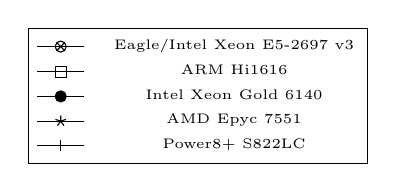
\begin{tikzpicture}[scale=1, baseline]
      \begin{customlegend}[legend columns=1,legend style={font=\tiny, column sep=2ex},
          legend entries={Eagle/Intel\ Xeon\ E5-2697 v3,
            ARM Hi1616,
            Intel\ Xeon\ Gold 6140,
            AMD Epyc 7551,
            Power8+ S822LC
        }]
        \addlegendimage{mark=otimes,solid}
        \addlegendimage{mark=square,solid}
        \addlegendimage{mark=*,solid}
        \addlegendimage{mark=star,solid}
        \addlegendimage{mark=|,solid}
      \end{customlegend}
    \end{tikzpicture}
  \end{subfigure}\hfill
  \begin{subfigure}[t]{0.48\textwidth}
    \centering
    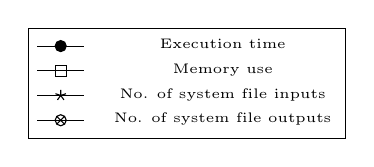
\begin{tikzpicture}[scale=1, baseline]
      \begin{customlegend}[legend columns=1,legend style={font=\tiny, column sep=2ex},
          legend entries={Execution time ,
            Memory use,
            No. of system file inputs,
            No. of system file outputs
        }]
        \addlegendimage{mark=*,solid}
        \addlegendimage{mark=square,solid}
        \addlegendimage{mark=star,solid}
        \addlegendimage{mark=otimes,solid}
      \end{customlegend}
    \end{tikzpicture}
  \end{subfigure}\bigbreak

  \begin{subfigure}[t]{0.48\textwidth}
    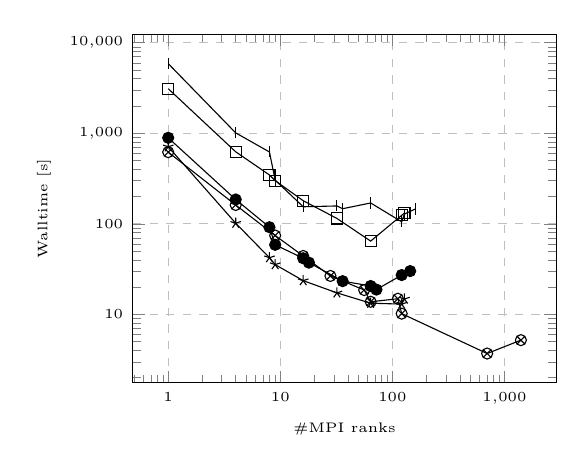
\begin{tikzpicture}[scale=1, baseline]
      \begin{axis}[
          xmode=log,
          ymode=log,
          log ticks with fixed point,
          scaled y ticks=real:1e3
          axis lines = left,
          xlabel = \#MPI ranks,
          ylabel = {Walltime [s]},
          legend style={at={(0.5,-0.2)},
            anchor=north,legend columns=1},
          xmajorgrids=true,
          ymajorgrids=true,
          grid style=dashed,
        ]
        %ARM
        \addplot [
          domain=1:150, 
          color=black,
          mark=square,
        ]
        coordinates {                 (1,3107.3)(4,624.3)(8,346.5)(9,299.7)(16,180.1)(32,114.7)(64,64.5)(121,124.3)(128,131.5)};
        %                \addlegendentry{ARM Hi1616}
        %Intel 6140
        \addplot [
          domain=1:150, 
          color=black,
          mark=*,
        ]
        coordinates {                   (1,891.2)(4,185.8)(8,91.8)(9,58.7)(16,41.7)(18,37.3)(36,23.3)(64,20.6)(72,18.8)(121,27.2)(144,30.1)};
        %                \addlegendentry{Intel\ Xeon\ Gold 6140}
        %AMD Epyc
        \addplot [
          domain=1:150, 
          color=black,
          mark=star,
        ]
        coordinates {
          (1,709.9)(4,101.6)(8,42.3)(9,35.5)(16,23.6)(32,17.3)(64,13.3)(121,13.0)(128,14.8)};
        %               \addlegendentry{AMD Epyc 7551}
        %Eagle
        \addplot [
          domain=1:1400, 
          color=black,
          mark=otimes,
        ]
        coordinates {                    (1,618.9)(4,161.5)(9,74.3)(16,44.2)(28,26.6)(56,18.6)(64,13.8)(112,14.9)(121,10.2)(700,3.7)(1400,5.2)
        };
        %               \addlegendentry{Eagle/Intel\ Xeon\ E5-2697 v3}
        %Power
        \addplot [
          domain=1:150, 
          color=black,
          mark=|,
        ]
        coordinates {
          (1,5878.0)(4,1010.5)(8,621.8)(9,304.1)(16,154.4)(32,157.6)(36,147)(64,170)(121,105.3)(128,128.3)(160,145.8)
        };
        %                \addlegendentry{Power8+ S822LC}
      \end{axis}
    \end{tikzpicture}
    \caption{IPF scalability}
    \label{fig:ipf_scalability}
  \end{subfigure}\hfill
  \begin{subfigure}[t]{0.48\textwidth}
    \centering
    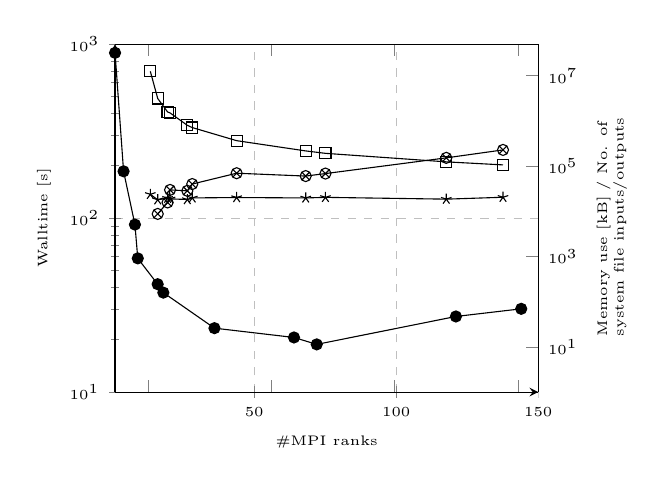
\begin{tikzpicture}[scale=1, baseline]
      \begin{axis}[
          %    width=1\textwidth,
          axis y line*=left,
          axis lines = left,
          xlabel = \#MPI ranks,
          ylabel = {Walltime [s]},
          xmajorgrids=true,
          ymajorgrids=true,
          grid style=dashed,
          xmin=1, xmax=150,
          ymode=log,
          ymin=10, ymax=1000,
        ]
        %Execution time
        \addplot [
          domain=1:70, 
          color=black,
          mark=*,
        ]
        coordinates {                   (1,891.2)(4,185.8)(8,91.8)(9,58.7)(16,41.7)(18,37.3)(36,23.3)(64,20.6)(72,18.8)(121,27.2)(144,30.1)};
        \label{ipf_execution_time}
      \end{axis}
      \begin{axis}[
          %                xmode=log,
          ymode=log,
          xticklabel=\empty,
          axis y line*=right,
          scaled ticks=false,
          y tick label style={/pgf/number format/.cd,sci,sci e},
          ymin=1, ymax=50000000,
          ylabel style={text width=3cm},
          ylabel = {Memory use {[kB]} {/} No. of system file inputs/outputs},
          legend style={at={(0.5,-0.2)},
            anchor=north,legend columns=1},
          grid style=dashed,
        ]
        \addlegendimage{/pgfplots/refstyle=ipf_execution_time}
        %                \addlegendentry{Execution time}
        %RAM
        \addplot [
          domain=1:70, 
          color=black,
          mark=square,
        ]
        coordinates {(1,12510916)(4,3140960)(8,1579868)(9,1505996)(16,800212)(18,713344)(36,365920)(64,216960)(72,191912)(121,124292)(144,106468)};
        %                \addlegendentry{Memory use}
        %#inputs
        \addplot [
          domain=1:70, 
          color=black,
          mark=star,
        ]
        coordinates {(1,23752)(4,18024)(8,19488)(9,18888)(16,18224)(18,19792)(36,20192)(64,19768)(72,20368)(121,18592)(144,20464)};
        %              \addlegendentry{No. of system file inputs}
        %#outputs
        \addplot [
          color=black,
          mark=otimes,
        ]
        coordinates {(1,0)(4,8760)(8,15728)(9,29744)(16,28400)(18,40128)(36,69664)(64,60248)(72,68416)(121,152384)(144,228360)};
        %                   \addlegendentry{No. of system file outputs}
      \end{axis}
    \end{tikzpicture}
    \caption{IPF on Intel\ Xeon\ Gold 6140}
    \label{fig:ipf_intel_gold}
  \end{subfigure}\bigbreak
  %      \caption{Results for IPF}
  %\end{figure}

  %% 3 row - \textsf{ABM4Py}
  %\begin{figure}[ht]
  %\centering
  \begin{subfigure}[t]{0.48\textwidth}
    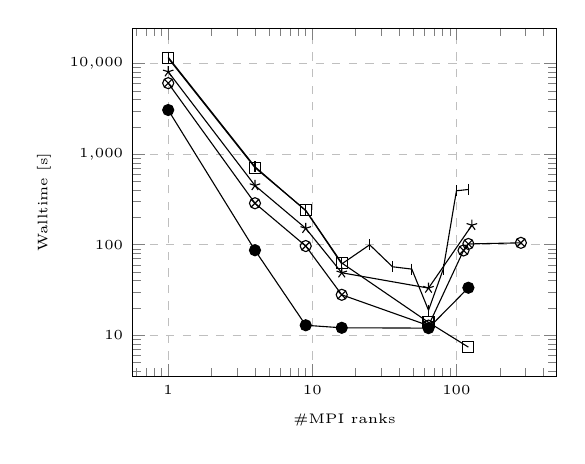
\begin{tikzpicture}[scale=1, baseline]
      \begin{axis}[
          xmode=log,
          ymode=log,
          log ticks with fixed point,
          scaled y ticks=real:1e3
          axis lines = left,
          xlabel = \#MPI ranks,
          ylabel = {Walltime [s]},
          %            legend style={at={(0.5,-0.2)},
          %            	    anchor=north,legend columns=1},
          xmajorgrids=true,
          ymajorgrids=true,
          grid style=dashed,
        ]
        %ARM
        \addplot [
          domain=1:150, 
          color=black,
          mark=square,
        ]
        coordinates {                 (1,11463.3)(4,708.9)(9,239.5)(16,62.9)(64,13.9)(121,7.4)};
        %                \addlegendentry{ARM Hi1616}
        %Intel 6140
        \addplot [
          domain=1:150, 
          color=black,
          mark=*,
        ]
        coordinates {                   (1,3071.5)(4,86.9)(9,12.9)(16,12.1)(64,12.0)(121,33.5)};
        %                \addlegendentry{Intel\ Xeon\ Gold 6140}
        %AMD Epyc
        \addplot [
          domain=1:150, 
          color=black,
          mark=star,
        ]
        coordinates {
          (1,8114.8)(4,450.3)(9,151.7)(16,49.0)(64,33.2)(128,164)};
        %                \addlegendentry{AMD Epyc 7551}
        %Eagle
        \addplot [
          domain=1:1400, 
          color=black,
          mark=otimes,
        ]
        coordinates {                    (1,6077.3)(4,287)(9,96.7)(16,28)(64,12.8)(112,86.4)(121,102)(280,104.9)
        };
        %                \addlegendentry{Eagle/Intel\ Xeon\ E5-2697 v3}
        %Power
        \addplot [
          domain=1:150, 
          color=black,
          mark=|,
        ]
        coordinates {
          (1,11751.7)(4,725.9)(9,237.9)(16,61.3)(25,99.8)(36,57.1)(49,53.8)(64,18.9)(81,53.7)(100,394.1)(121,407.3)
        };
        %                \addlegendentry{Power8+ S822LC}
      \end{axis}
    \end{tikzpicture}
    \caption{\textsf{ABM4Py}/GG scalability}
    \label{fig:abms_scalability}
  \end{subfigure}\hfill
  \begin{subfigure}[t]{0.48\textwidth}
    \centering
    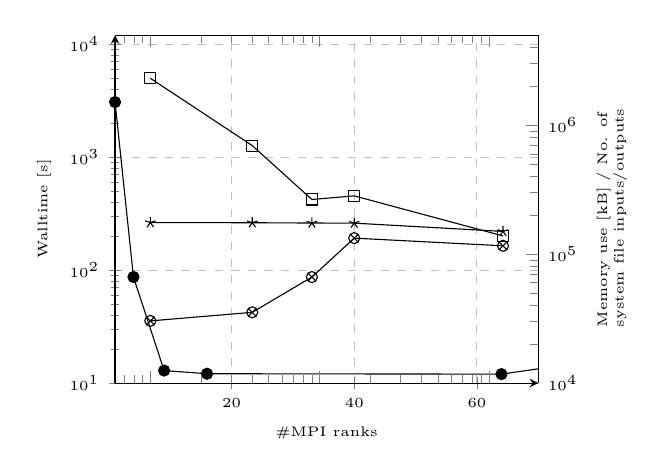
\begin{tikzpicture}[scale=1, baseline]
      \begin{axis}[
          %    width=1\textwidth,
          axis y line*=left,
          axis lines = left,
          xlabel = \#MPI ranks,
          ylabel = {Walltime [s]},
          xmajorgrids=true,
          ymajorgrids=true,
          grid style=dashed,
          xmin=1, xmax=70,
          ymode=log,
          ymin=10, ymax=12000,
        ]
        %Execution time
        \addplot [
          domain=1:70, 
          color=black,
          mark=*,
        ]
        coordinates {                   (1,3071.5)(4,86.9)(9,12.9)(16,12.1)(64,12.0)(121,33.5)};
        \label{abms_execution_time}
      \end{axis}
      \begin{axis}[
          xmode=log,
          ymode=log,
          xticklabel=\empty,
          axis y line*=right,
          scaled ticks=false,
          y tick label style={/pgf/number format/.cd,sci,sci e},
          ymin=10000, ymax=5000000,
          ylabel style={text width=3cm},
          ylabel = {Memory use {[kB]} {/} No. of system file inputs/outputs},
          %                legend style={at={(0.5,-0.2)},
          %                	    anchor=north,legend columns=1},
          grid style=dashed,
        ]
        \addlegendimage{/pgfplots/refstyle=abms_execution_time}
        %                \addlegendentry{Execution time}
        %RAM
        \addplot [
          domain=1:70, 
          color=black,
          mark=square,
        ]
        coordinates {(1,2316696)(4,695464)(9,265676)(16,283352)(121,138564)};
        %              \addlegendentry{Memory use}
        %#inputs
        \addplot [
          domain=1:70, 
          color=black,
          mark=star,
        ]
        coordinates {(1,175888)(4,175368)(9,174456)(16,174088)(121,150160)};
        %               \addlegendentry{No. of system file inputs}
        %#outputs
        \addplot [
          color=black,
          mark=otimes,
        ]
        coordinates {(1,30360)(4,35384)(9,66448)(16,133160)(121,116104)};
        %                    \addlegendentry{No. of system file outputs}
      \end{axis}
    \end{tikzpicture}
    \caption{\textsf{ABM4Py}/GG Intel\ Xeon\ Gold 6140}
    \label{fig:abms_intel_gold}
  \end{subfigure}\bigbreak

  
  %% 2 row - \textsf{Pandora}/GG
  %\begin{figure}[ht]
  %\centering
  \begin{subfigure}[t]{0.48\textwidth}
    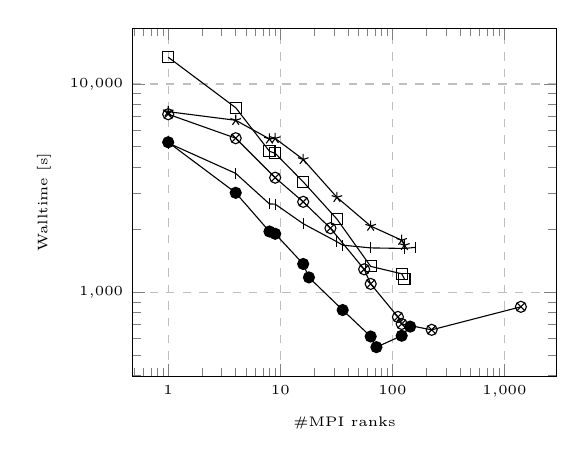
\begin{tikzpicture}[scale=1, baseline]
      \begin{axis}[
          xmode=log,
          ymode=log,
          log ticks with fixed point,
          scaled y ticks=real:1e3
          axis lines = left,
          xlabel = \#MPI ranks,
          ylabel = {Walltime [s]},
          %            legend style={at={(0.5,-0.2)},
          %            	    anchor=north,legend columns=1},
          xmajorgrids=true,
          ymajorgrids=true,
          grid style=dashed,
        ]
        %ARM
        \addplot [
          domain=1:150, 
          color=black,
          mark=square,
        ]
        coordinates {                 (1,13437.4)(4,7694.2)(8,4756.2)(9,4647.5)(16,3393.4)(32,2249)(64,1333.4)(121,1229.1)(128,1161.9)};
        %                \addlegendentry{ARM Hi1616}
        %Intel 6140
        \addplot [
          domain=1:150, 
          color=black,
          mark=*,
        ]
        coordinates {                   (1,5253.9)(4,3005.9)(8,1960.8)(9,1911.8)(16,1369.7)(18,1180.8)(36,823.6)(64,614.9)(72,546.6)(121,620.0)(144,685.8)};
        %                \addlegendentry{Intel\ Xeon\ Gold 6140}
        %AMD Epyc
        \addplot [
          domain=1:150, 
          color=black,
          mark=star,
        ]
        coordinates {
          (1,7364.1)(4,6696.0)(8,5451.3)(9,5480)(16,4345.6)(32,2859.2)(64,2081.9)(121,1781.2)(128,1683.8)};
        %               \addlegendentry{AMD Epyc 7551}
        %Eagle
        \addplot [
          domain=1:1400, 
          color=black,
          mark=otimes,
        ]
        coordinates {                    (1,7158.7)(4,5493.6)(9,3552.1)(16,2720.5)(28,2033)(56,1291.2)(64,1099.1)(112,763.1)(121,706.3)(224,661.7)(1400,853.4)
        };
        %                \addlegendentry{Eagle/Intel\ Xeon\ E5-2697 v3}
        %Power
        \addplot [
          domain=1:150, 
          color=black,
          mark=|,
        ]
        coordinates {
          (1,5208.5)(4,3725.4)(8,2658.6)(9,2652.2)(16,2137.1)(32,1750.5)(36,1686.2)(64,1635.6)(128,1625.7)(160,1644.8)
        };
        %                \addlegendentry{Power8+ S822LC}
      \end{axis}
    \end{tikzpicture}
    \caption{\textsf{Pandora}/GG scalability}
    \label{fig:pandora_scalability}
  \end{subfigure}\hfill
  \begin{subfigure}[t]{0.48\textwidth}
    \centering
    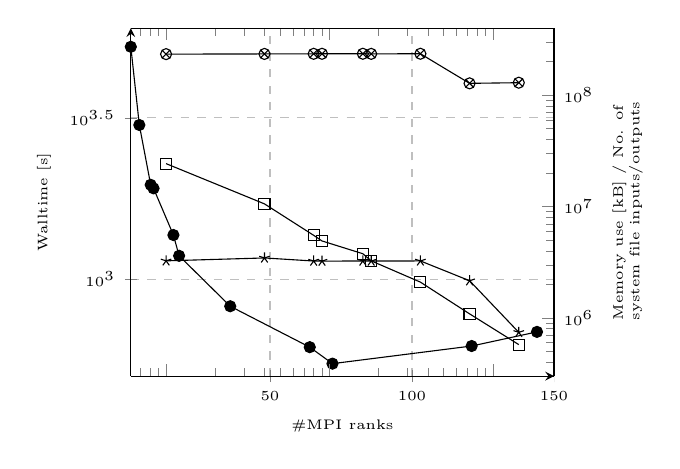
\begin{tikzpicture}[scale=1, baseline]
      \begin{axis}[
          %    width=1\textwidth,
          axis y line*=left,
          axis lines = left,
          xlabel = \#MPI ranks,
          ylabel = {Walltime [s]},
          xmajorgrids=true,
          ymajorgrids=true,
          grid style=dashed,
          xmin=1, xmax=150,
          ymode=log,
          ymin=500, ymax=6000,
        ]
        %Execution time
        \addplot [
          domain=1:70, 
          color=black,
          mark=*,
        ]
        coordinates {                   (1,5253.9)(4,3005.9)(8,1960.8)(9,1911.8)(16,1369.7)(18,1180.8)(36,823.6)(64,614.9)(72,546.6)(121,620.0)(144,685.8)};
        \label{pandora_execution_time}
      \end{axis}
      \begin{axis}[
          xmode=log,
          ymode=log,
          xticklabel=\empty,
          axis y line*=right,
          scaled ticks=false,
          y tick label style={/pgf/number format/.cd,sci,sci e},
          ymin=300000, ymax=400000000,
          ylabel style={text width=3cm},
          ylabel = {Memory use {[kB]} {/} No. of system file inputs/outputs},
          legend style={at={(0.5,-0.2)},
            anchor=north,legend columns=1},
          grid style=dashed,
        ]
        \addlegendimage{/pgfplots/refstyle=pandora_execution_time}
        %                \addlegendentry{Execution time}
        %RAM
        \addplot [
          domain=1:70, 
          color=black,
          mark=square,
        ]
        coordinates {(1,24316736)(4,10578468)(8,5519380)(9,4912336)(16,3772628)(18,3255200)(36,2096424)(72,1087508)(144,575948)};
        %               \addlegendentry{Memory use}
        %#inputs
        \addplot [
          domain=1:70, 
          color=black,
          mark=star,
        ]
        coordinates {(1,3255992)(4,3455808)(8,3243280)(9,3237968)(16,3245208)(18,3244448)(36,3249248)(72,2158432)(144,742416)};
        %               \addlegendentry{No. of system file inputs}
        %#outputs
        \addplot [
          color=black,
          mark=otimes,
        ]
        coordinates {(1,234115384)(4,235057696)(8,235684024)(9,235765544)(16,235883464)(18,235413696)(36,235913920)(72,127931040)(144,129657720)};
        %                    \addlegendentry{No. of system file outputs}
      \end{axis}
    \end{tikzpicture}
    \caption{\textsf{Pandora}/GG on Intel\ Xeon\ Gold 6140}
    \label{fig:pandora_intel_gold}
  \end{subfigure}\bigbreak
  %      \caption{Results for \textsf{Pandora}/GG (worldwide map)}
  %\end{figure}

  \caption{Results for social simulation applications}
  \label{fig:socapps_plots}
\end{figure}

%% 1 row - OpenSWPC
\begin{figure}[tphb]
  \centering
  \iffalse
  \begin{subfigure}[t]{0.48\textwidth}
    \centering
    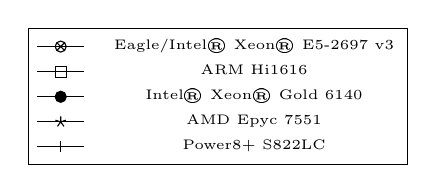
\begin{tikzpicture}[scale=1, baseline]
      \begin{customlegend}[legend columns=1,legend style={font=\tiny, column sep=2ex},
          legend entries={Eagle/Intel\textregistered\ Xeon\textregistered\ E5-2697 v3,
            ARM Hi1616,
            Intel\textregistered\ Xeon\textregistered\ Gold 6140,
            AMD Epyc 7551,
            Power8+ S822LC
        }]
        \addlegendimage{mark=otimes,solid}
        \addlegendimage{mark=square,solid}
        \addlegendimage{mark=*,solid}
        \addlegendimage{mark=star,solid}
        \addlegendimage{mark=|,solid}
      \end{customlegend}
    \end{tikzpicture}
  \end{subfigure}\hfill
  \begin{subfigure}[t]{0.48\textwidth}
    \centering
    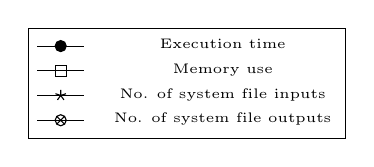
\begin{tikzpicture}[scale=1, baseline]
      \begin{customlegend}[legend columns=1,legend style={font=\tiny, column sep=2ex},
          legend entries={Execution time ,
            Memory use,
            No. of system file inputs,
            No. of system file outputs
        }]
        \addlegendimage{mark=*,solid}
        \addlegendimage{mark=square,solid}
        \addlegendimage{mark=star,solid}
        \addlegendimage{mark=otimes,solid}
      \end{customlegend}
    \end{tikzpicture}
  \end{subfigure}\bigbreak
  \fi
  \begin{subfigure}[t]{0.48\textwidth}
    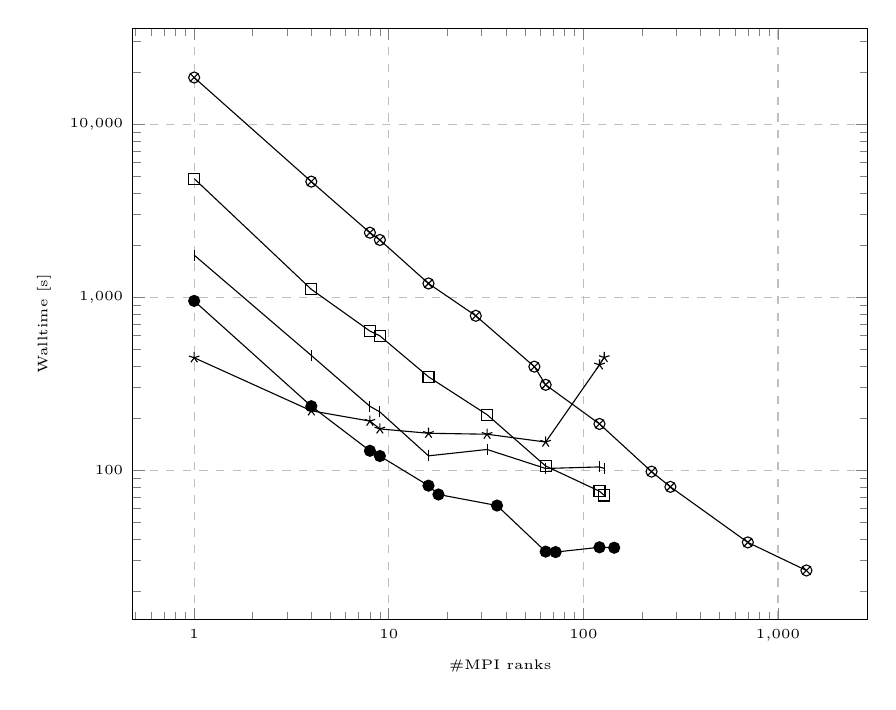
\begin{tikzpicture}[scale=1, baseline]
      \begin{axis}[width=.9\textwidth,height=.75\textwidth,
          xmode=log,
          ymode=log,
          log ticks with fixed point,
          scaled y ticks=real:1e3
          axis lines = left,
          xlabel = \#MPI ranks,
          ylabel = {Walltime [s]},
          %            legend style={at={(0.5,-0.2)},
          %            	    anchor=north,legend columns=1},
          xmajorgrids=true,
          ymajorgrids=true,
          grid style=dashed,
        ]
        %ARM
        \addplot [
          domain=1:150, 
          color=black,
          mark=square,
        ]
        coordinates {
          (1,4840)(4,1109)(8,636.4)(9,596.9)(16,346.1)(32,209.1)(64,105.6)(121,75.5)(128,71.4)
        };
        %                \addlegendentry{ARM Hi1616}
        %Intel 6140
        \addplot [
          domain=1:150, 
          color=black,
          mark=*,
        ]
        coordinates {
          (1,950.4)(4,234)(8,129.3)(9,120.6)(16,81.3)(18,72.3)(36,62.4)(64,33.8)(72,33.6)(121,35.8)(144,35.6)
        };
        %               \addlegendentry{Intel\textregistered\ Xeon\textregistered\ Gold 6140}
        %AMD Epyc
        \addplot [
          domain=1:150, 
          color=black,
          mark=star,
        ]
        coordinates {
          (1,446.1)(4,220.2)(8,192)(9,173)(16,163.3)(32,161.21)(64,145.3)(121,406)(128,448.1)
        };
        %               \addlegendentry{AMD Epyc 7551}
        %Eagle
        \addplot [
          domain=1:1400, 
          color=black,
          mark=otimes,
        ]
        coordinates {                    (1,18584.8)(4,4649.8)(8,2356.4)(9,2139.0)(16,1198.7)(28,779.8)(56,396.2)(64,311.1)(121,184.9)(224,98)(280,80)(700,38.2)(1400,26.3)
        };
        %              \addlegendentry{Eagle/Intel\textregistered\ Xeon\textregistered\ E5-2697 v3}
        %Power
        \addplot [
          domain=1:150, 
          color=black,
          mark=|,
        ]
        coordinates {
          (1,1748.7)(4,459.8)(8,233.7)(9,216.9)(16,120.9)(32,131.6)(64,102.2)(121,104.3)(128,102.2)
        };
        %                \addlegendentry{Power8+ S822LC}
      \end{axis}
    \end{tikzpicture}
    \caption{OpenSWPC scalability}
    \label{fig:openswpc_scalability}
  \end{subfigure}\hfill
  \begin{subfigure}[t]{0.48\textwidth}
    \centering
    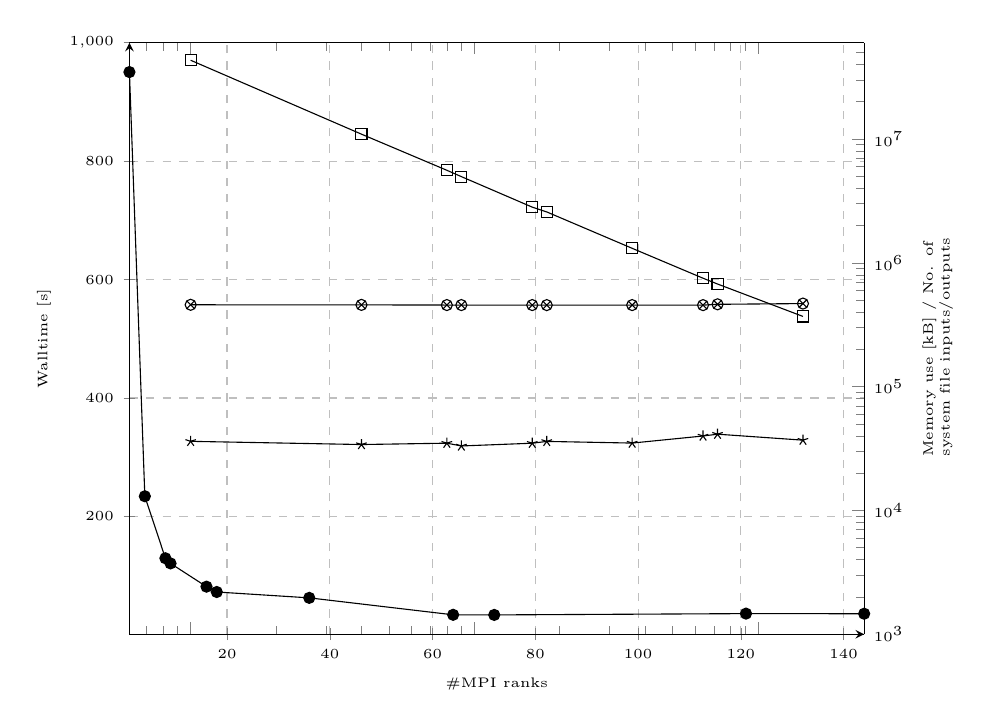
\begin{tikzpicture}[scale=1, baseline]
      \begin{axis}[width=.9\textwidth,height=.75\textwidth,
          %    width=1\textwidth,
          axis y line*=left,
          axis lines = left,
          xlabel = \#MPI ranks,
          ylabel = {Walltime [s]},
          xmajorgrids=true,
          ymajorgrids=true,
          grid style=dashed,
          ymin=1, ymax=1000,
        ]
        %Execution time
        \addplot [
          domain=1:70, 
          color=black,
          mark=*,
        ]
        coordinates {(1,950.4)(4,234)(8,129.3)(9,120.6)(16,81.3)(18,72.3)(36,62.4)(64,33.8)(72,33.6)(121,35.8)(144,35.6)};
        \label{openswpc_execution_time}
      \end{axis}
      \begin{axis}[width=.9\textwidth,height=.75\textwidth,
          xmode=log,
          ymode=log,
          xticklabel=\empty,
          axis y line*=right,
          scaled ticks=false,
          y tick label style={/pgf/number format/.cd,sci,sci e},
          ymin=1000, ymax=60000000,
          ylabel style={text width=3cm},
          ylabel = {Memory use {[kB]} {/} No. of system file inputs/outputs},
          legend style={at={(0.5,-0.2)},
            anchor=north,legend columns=1},
          grid style=dashed,
        ]
        \addlegendimage{/pgfplots/refstyle=openswpc_execution_time}
        %                \addlegendentry{Execution time}
        %RAM
        \addplot [
          domain=1:70, 
          color=black,
          mark=square,
        ]
        coordinates {(1,43267296)(4,10943064)(8,5590132)(9,4967892)(16,2816788)(18,2576328)(36,1309532)(64,751016)(72,674056)(144,368968)};
        %                \addlegendentry{Memory use}
        %#inputs
        \addplot [
          domain=1:70, 
          color=black,
          mark=star,
        ]
        coordinates {(1,36144)(4,34048)(8,34920)(9,33160)(16,34896)(18,36088)(36,34992)(64,39920)(72,41272)(144,36944)};
        %               \addlegendentry{No. of system file inputs}
        %#outputs
        \addplot [
          color=black,
          mark=otimes,
        ]
        coordinates {(1,458040)(4,457256)(8,455752)(9,455664)(16,455688)(18,455248)(36,455544)(64,455168)(72,462144)(144,468512)};
        %                    \addlegendentry{No. of system file outputs}
      \end{axis}
    \end{tikzpicture}
    \caption{OpenSWPC on Intel Xeon Gold 6140}
    \label{fig:openswpc_intel_gold}
  \end{subfigure}\bigbreak
  %      \caption{Results for OpenSWPC}
  %\end{figure}


  %%2 row - CMAQ/CCTM
  %\begin{figure}[ht]
  %\centering
  \begin{subfigure}[t]{0.48\textwidth}
    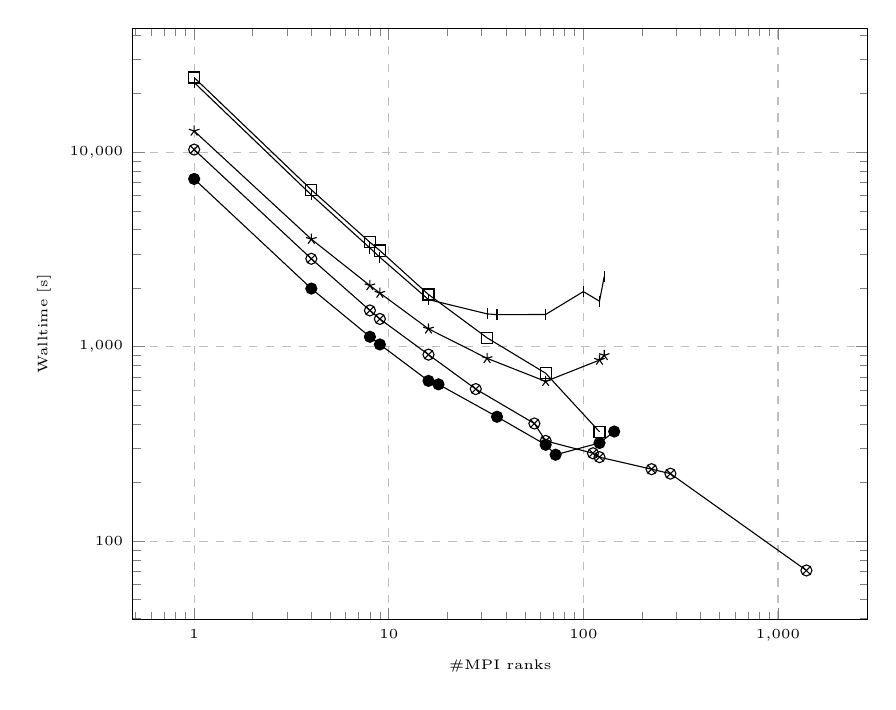
\begin{tikzpicture}[scale=1, baseline]
      \begin{axis}[width=.9\textwidth,height=.75\textwidth,
          %    width=1.3\textwidth,
          xmode=log,
          ymode=log,
          log ticks with fixed point,
          scaled y ticks=real:1e3
          axis lines = left,
          xlabel = \#MPI ranks,
          ylabel = {Walltime [s]},
          %        legend style={at={(0.5,-0.2)},
          %        	    anchor=north,legend columns=1},
          xmajorgrids=true,
          ymajorgrids=true,
          grid style=dashed,
        ]
        %ARM
        \addplot [
          domain=1:150, 
          color=black,
          mark=square,
        ]
        coordinates {
          (1,24239.6)(4,6416.1)(8,3445.6)(9,3124.6)(16,1856.3)(32,1111.4)(64,730.7)(121,365.4)
        };
        %        \addlegendentry{ARM Hi1616}
        %Intel 6140
        \addplot [
          domain=1:150, 
          color=black,
          mark=*,
        ]
        coordinates {
          (1,7294.6)(4,1991.6)(8,1125.1)(9,1027.3)(16,667.5)(18,640.7)(36,436.4)(64,313.2)(72,278.4)(121,320)(144,366.5)
        };
        %        \addlegendentry{Intel\textregistered\ Xeon\textregistered\ Gold 6140}
        %AMD Epyc
        \addplot [
          domain=1:150, 
          color=black,
          mark=star,
        ]
        coordinates {
          (1,12872.6)(4,3574.8)(8,2064.3)(9,1888.6)(16,1235.9)(32,871.8)(64,663.3)(121,853.9)(128,902.9)
        };
        %        \addlegendentry{AMD Epyc 7551}
        %Eagle
        \addplot [
          domain=1:1400,
          color=black,
          mark=otimes,
        ]
        coordinates {
          (1,10323.7)(4,2834.3)(8,1537)(9,1389.7)(16,910.7)(28,605.8)(56,402.9)(64,327.9)(112,283.3)(121,270.5)(224,234.6)(280,222.5)(1400,70.7)
        };
        %       \addlegendentry{Eagle/Intel\textregistered\ Xeon\textregistered\ E5-2697 v3}
        %Power
        \addplot [
          domain=1:150, 
          color=black,
          mark=|,
        ]
        coordinates {
          (1,22849.8)(4,6036.1)(8,3220.3)(9,2885.9)(16,1748.2)(32,1476)(36,1461.4)(64,1465.4)(100,1921.8)(121,1714.5)(128,2297.7)
        };
        %      \addlegendentry{Power8+ S822LC}
      \end{axis}
    \end{tikzpicture}
    \caption{CMAQ/CCTM scalability}
    \label{fig:cmaq_scalability}
  \end{subfigure}\hfill
  \begin{subfigure}[t]{0.48\textwidth}
    \centering
    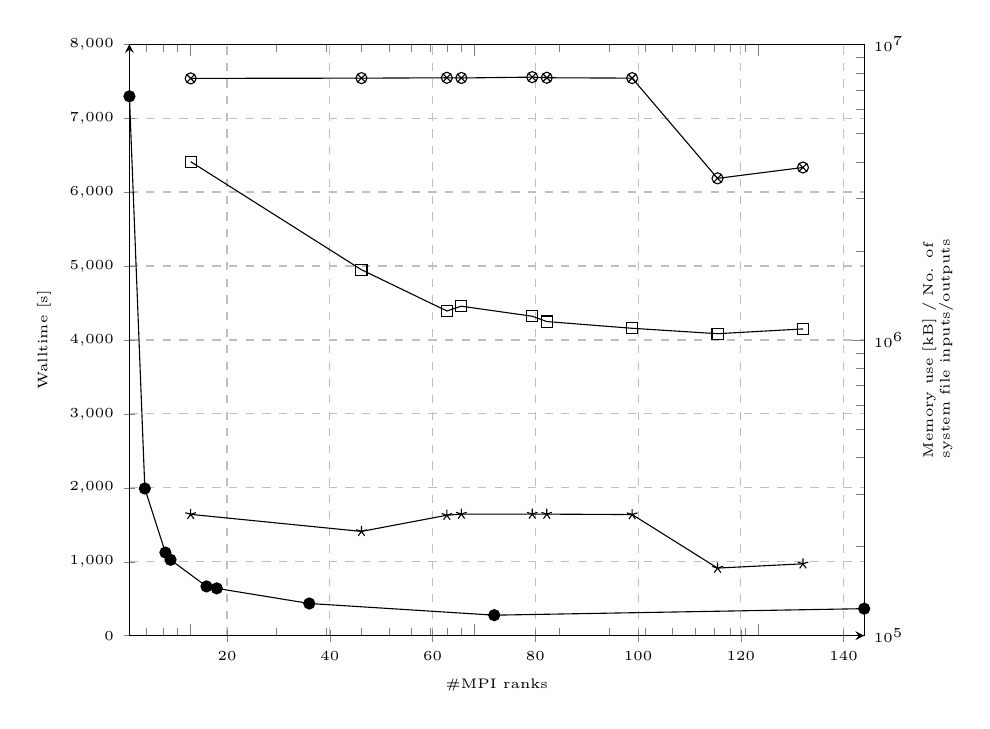
\begin{tikzpicture}[scale=1, baseline]
      \begin{axis}[width=.9\textwidth,height=.75\textwidth,
          %    width=1\textwidth,
          axis y line*=left,
          axis lines = left,
          xlabel = \#MPI ranks,
          ylabel = {Walltime [s]},
          xmajorgrids=true,
          ymajorgrids=true,
          grid style=dashed,
          ymin=1, ymax=8000,
        ]
        %Execution time
        \addplot [
          domain=1:70, 
          color=black,
          mark=*,
        ]
        coordinates {(1,7294.6)(4,1991.4)(8,1125.1)(9,1027.3)(16,667.5)(18,640.7)(36,436.4)(72,278.4)(144,366.5)};
        \label{cmaq_execution_time}
      \end{axis}
      \begin{axis}[width=.9\textwidth,height=.75\textwidth,
          xmode=log,
          ymode=log,
          xticklabel=\empty,
          axis y line*=right,
          scaled ticks=false,
          y tick label style={/pgf/number format/.cd,sci,sci e},
          ymin=100000, ymax=10000000,
          ylabel style={text width=3cm},
          ylabel = {Memory use {[kB]} {/} No. of system file inputs/outputs},
          %                legend style={at={(0.5,-0.2)},
          %                	    anchor=north,legend columns=1},
          grid style=dashed,
        ]
        \addlegendimage{/pgfplots/refstyle=cmaq_execution_time}
        %                \addlegendentry{Execution time}
        %RAM
        \addplot [
          domain=1:70, 
          color=black,
          mark=square,
        ]
        coordinates {(1,4005556)(4,1726776)(8,1252488)(9,1299756)(16,1202224)(18,1153424)(36,1094592)(72,1049436)(144,1089048)};
        %                \addlegendentry{Memory use}
        %#inputs
        \addplot [
          domain=1:70, 
          color=black,
          mark=star,
        ]
        coordinates {(1,257120)(4,225160)(8,255344)(9,257736)(16,257736)(18,257592)(36,256752)(72,169256)(144,174968)};
        %               \addlegendentry{No. of system file inputs}
        %#outputs
        \addplot [
          color=black,
          mark=otimes,
        ]
        coordinates {(1,7660576)(4,7674568)(8,7695080)(9,7684712)(16,7735376)(18,7696800)(36,7676016)(72,3516968)(144,3827848)};
        %                \addlegendentry{No. of system file outputs}
      \end{axis}
    \end{tikzpicture}
    %          \caption{CMAQ/CCTM detailed results for Intel\textregistered\ Xeon\textregistered\ Gold 6140}
    \caption{CMAQ/CCTM on Intel Xeon Gold 6140}
    \label{fig:cmaq_intel_gold}
  \end{subfigure}\bigbreak
  %    \caption{Results for CMAQ/CCTM}


  %%3 row - CM1

  \begin{subfigure}[t]{0.48\textwidth}
    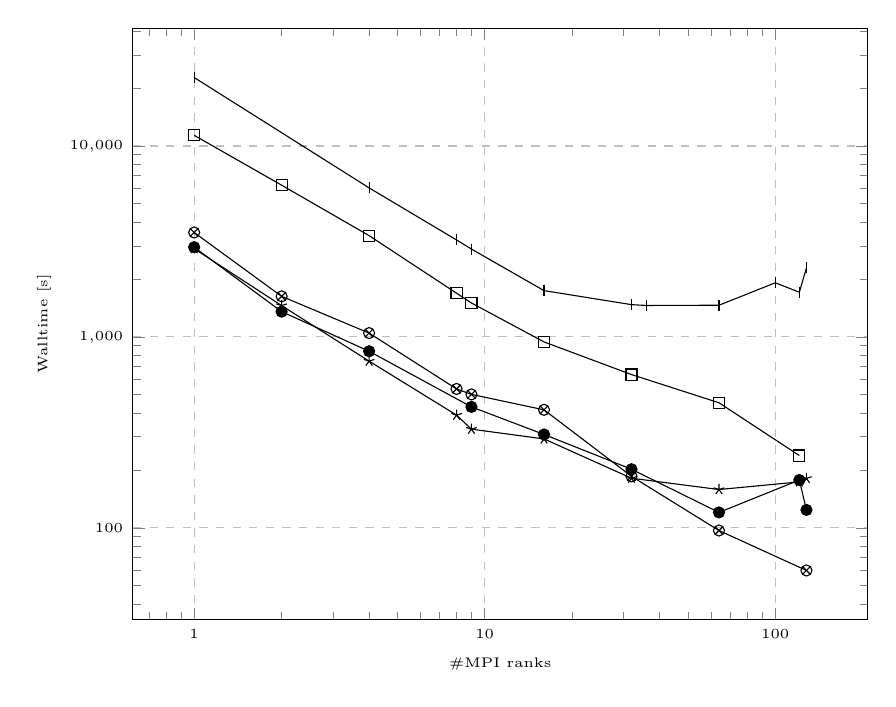
\begin{tikzpicture}[scale=1, baseline]
      \begin{axis}[width=.9\textwidth,height=.75\textwidth,
          xmode=log,
          ymode=log,
          log ticks with fixed point,
          scaled y ticks=real:1e3
          axis lines = left,
          xlabel = \#MPI ranks,
          ylabel = {Walltime [s]},
          %            legend style={at={(0.5,-0.2)},
          %            	    anchor=north,legend columns=1},
          xmajorgrids=true,
          ymajorgrids=true,
          grid style=dashed,
        ]
        %ARM
        \addplot [
          domain=1:150, 
          color=black,
          mark=square,
        ]
        coordinates {
          (1,11379.8)(2,6236)(4,3393.1)(8,1694.1)(9,1505.9)(16,941.5)(32,635.1)(64,452)(121,239.1)
        };
        %           \addlegendentry{ARM Hi1616}
        %Intel 6140
        \addplot [
          domain=1:150, 
          color=black,
          mark=*,
        ]
        coordinates {
          (1,2952)(2,1356.7)(4,841.2)(9,430)(16,308.4)(32,202.7)(64,120.4)(121,178)(128,124.1)
        };
        %          \addlegendentry{Intel\textregistered\ Xeon\textregistered\ Gold 6140}
        %AMD Epyc
        \addplot [
          domain=1:150, 
          color=black,
          mark=star,
        ]
        coordinates {
          (1,2900)(2,1459)(4,746.8)(8,389.4)(9,328.7)(16,292.2)(32,181.9)(64,158.7)(121,174)(128,181.5)
        };
        %            \addlegendentry{AMD Epyc 7551}
        %Eagle
        \addplot [
          domain=1:1400,
          color=black,
          mark=otimes,
        ]
        coordinates {
          (1,3524)(2,1631.4)(4,1047.2)(8,534)(9,500)(16,415)(32,186.1)(64,96.8)(128,59.8)
        };
        %           \addlegendentry{Eagle/Intel\textregistered\ Xeon\textregistered\ E5-2697 v3}
        %Power
        \addplot [
          domain=1:150, 
          color=black,
          mark=|,
        ]
        coordinates {
          (1,22849.8)(4,6036.1)(8,3220.3)(9,2885.9)(16,1748.2)(32,1476)(36,1461.4)(64,1465.4)(100,1921.8)(121,1714.5)(128,2297.7)
        };
        %          \addlegendentry{Power8+ S822LC}
      \end{axis}
    \end{tikzpicture}
    \caption{CM1\ scalability}
    \label{fig:cm1_scalability}
  \end{subfigure}\hfill
  \begin{subfigure}[t]{0.48\textwidth}
    \centering
    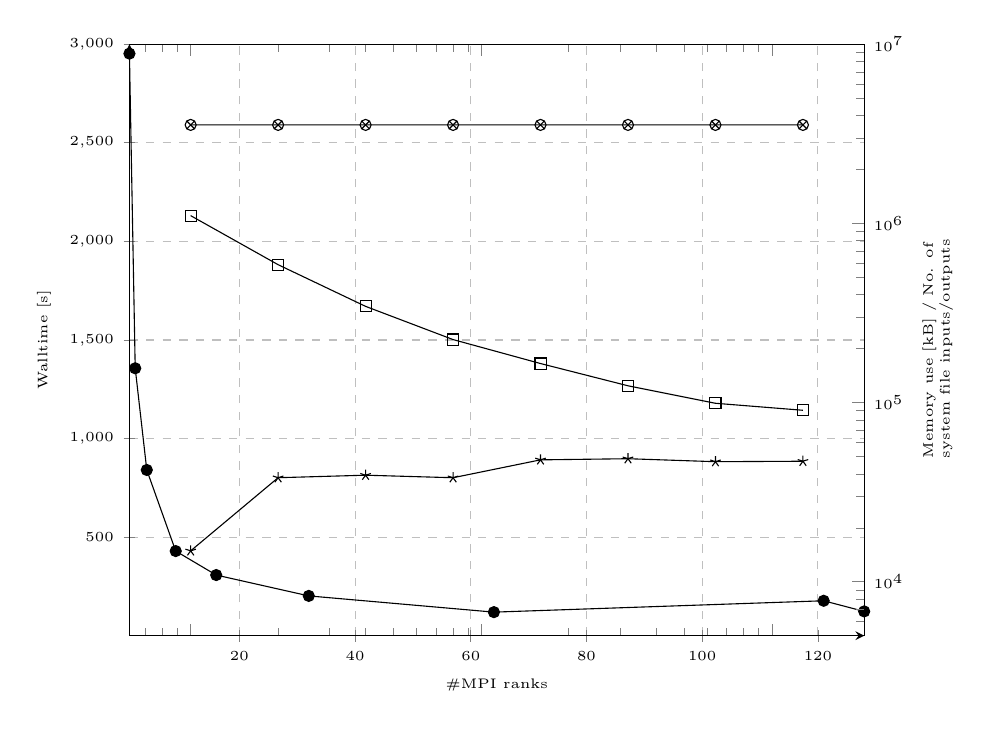
\begin{tikzpicture}[scale=1, baseline]
      \begin{axis}[width=.9\textwidth,height=.75\textwidth,
          %    width=1\textwidth,
          axis y line*=left,
          axis lines = left,
          xlabel = \#MPI ranks,
          ylabel = {Walltime [s]},
          xmajorgrids=true,
          ymajorgrids=true,
          grid style=dashed,
          ymin=1, ymax=3000,
        ]
        %Execution time
        \addplot [
          domain=1:70, 
          color=black,
          mark=*,
        ]
        coordinates {
          (1,2952)(2,1356.7)(4,841.2)(9,430)(16,308.4)(32,202.7)(64,120.4)(121,178)(128,124.1)};
        \label{cm1_execution_time}
      \end{axis}
      \begin{axis}[width=.9\textwidth,height=.75\textwidth,
          xmode=log,
          ymode=log,
          xticklabel=\empty,
          axis y line*=right,
          scaled ticks=false,
          y tick label style={/pgf/number format/.cd,sci,sci e},
          ymin=5000, ymax=10000000,
          ylabel style={text width=3cm},
          ylabel = {Memory use {[kB]} {/} No. of system file inputs/outputs
          },
          legend style={at={(0.5,-0.2)},
            anchor=north,legend columns=1},
          grid style=dashed,
        ]
        \addlegendimage{/pgfplots/refstyle=cm1_execution_time}
        %            \addlegendentry{Execution time}
        %RAM
        \addplot [
          domain=1:70, 
          color=black,
          mark=square,
        ]
        coordinates {(1,1104060)(2,587776)(4,344076)(8,224576)(16,165060)(32,124016)(64,99052)(128,90536)};
        %            \addlegendentry{Memory use}
        %#inputs
        \addplot [
          domain=1:70, 
          color=black,
          mark=star,
        ]
        coordinates {(1,14872)(2,38064)(4,39312)(8,38056)(16,47880)(32,48584)(64,46760)(128,47032)};
        %           \addlegendentry{No. of system file inputs}
        %#outputs
        \addplot [
          color=black,
          mark=otimes,
        ]
        coordinates {(1,3542800)(2,3542536)(4,3542224)(8,3541976)(16,3541912)(32,3541784)(64,3541336)(128,3541336)};
        %            \addlegendentry{No. of system file outputs}
      \end{axis}
    \end{tikzpicture}
    %  \caption{CM1 detailed results for Intel\textregistered\ Xeon\textregistered\ Gold 6140}
    \caption{CM1 on Intel Xeon Gold 6140}
    \label{fig:cm1_intel_gold}
  \end{subfigure}%
  %  \caption{Results for CM1}
  %\end{figure}

  %%4 row - HWRF
  %\begin{figure}[ht]
  \begin{subfigure}[t]{0.48\textwidth}
    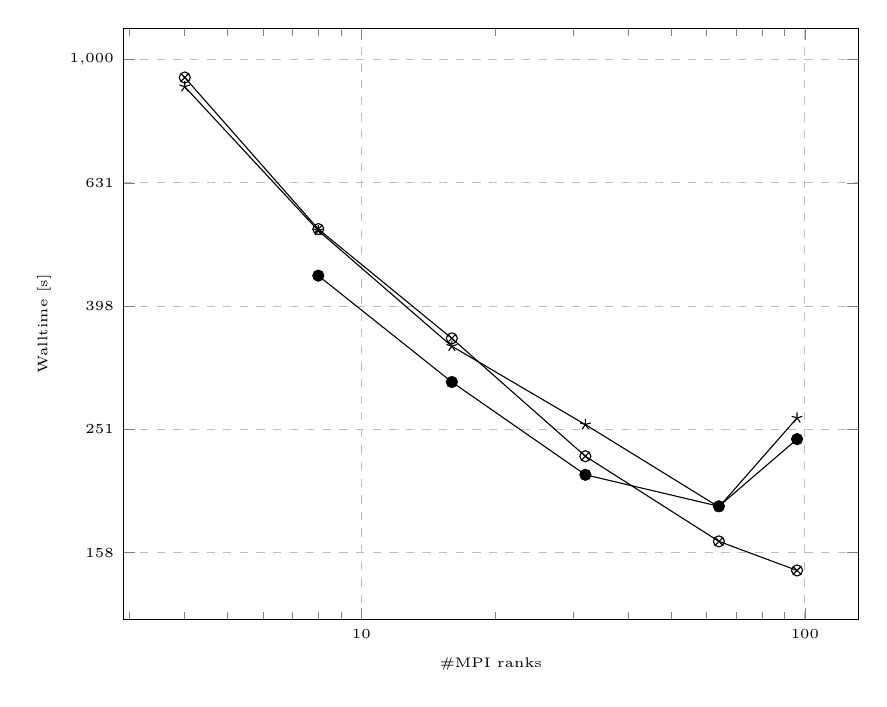
\begin{tikzpicture}[scale=1, baseline]
      \begin{axis}[width=.9\textwidth,height=.75\textwidth,
          xmode=log,
          ymode=log,
          log ticks with fixed point,
          scaled y ticks=real:1e3
          axis lines = left,
          xlabel = \#MPI ranks,
          ylabel = {Walltime [s]},
          %           legend style={at={(0.5,-0.2)},
          %            	    anchor=north,legend columns=1},
          xmajorgrids=true,
          ymajorgrids=true,
          grid style=dashed,
        ]
        %Intel 6140
        \addplot [
          domain=1:150, 
          color=black,
          mark=*,
        ]
        coordinates {(8,446)(16,299.8)(32,212)(64,188.5)(96,242.2)};
        %           \addlegendentry{Intel\textregistered\ Xeon\textregistered\ Gold 6140}
        %AMD Epyc
        \addplot [
          domain=1:150, 
          color=black,
          mark=star,
        ]
        coordinates {
          (4,903.4)(8,527.7)(16,342.7)(32,255.7)(64,188)(96,262.1)
        };
        %          \addlegendentry{AMD Epyc 7551}
        %Eagle
        \addplot [
          domain=1:1400,
          color=black,
          mark=otimes,
        ]
        coordinates {
          (4,935)(8,530.8)(16,352.9)(32,227.2)(64,165.3)(96,148.3)                };
        %          \addlegendentry{Eagle/Intel\textregistered\ Xeon\textregistered\ E5-2697 v3}
      \end{axis}
    \end{tikzpicture}
    \caption{HWRF\ scalability}
    \label{fig:hwrf_scalability}
  \end{subfigure}\hfill
  \begin{subfigure}[t]{0.48\textwidth}
    \centering
    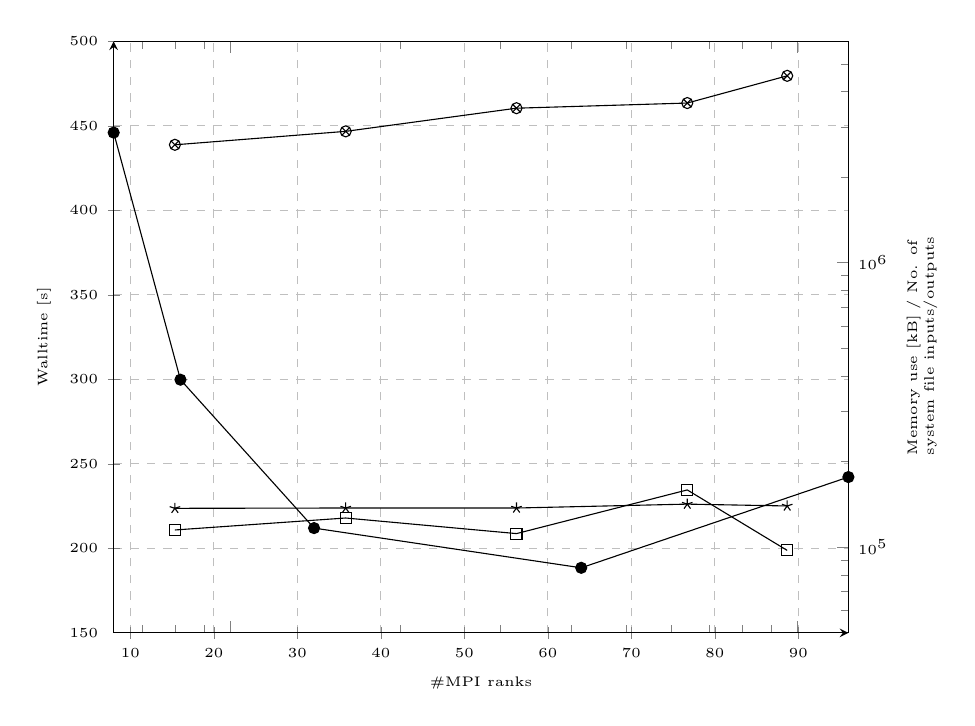
\begin{tikzpicture}[scale=1, baseline]
      \begin{axis}[width=.9\textwidth,height=.75\textwidth,
          axis y line*=left,
          axis lines = left,
          xlabel = \#MPI ranks,
          ylabel = {Walltime [s]},
          xmajorgrids=true,
          ymajorgrids=true,
          grid style=dashed,
          ymin=150, ymax=500,
        ]
        %Execution time
        \addplot [
          domain=1:70, 
          color=black,
          mark=*,
        ]
        coordinates {(8,446)(16,299.8)(32,212)(64,188.5)(96,242.2)};
        \label{hwrf_execution_time}
      \end{axis}
      \begin{axis}[width=.9\textwidth,height=.75\textwidth,
          xmode=log,
          ymode=log,
          xticklabel=\empty,
          axis y line*=right,
          scaled ticks=false,
          y tick label style={/pgf/number format/.cd,sci,sci e},
          ymin=50000, ymax=6000000,
          ylabel style={text width=3cm},
          ylabel = {Memory use {[kB]} {/} No. of system file inputs/outputs
          },
          %            legend style={at={(0.5,-0.2)},
          %            	    anchor=north,legend columns=1},
          grid style=dashed,
        ]
        \addlegendimage{/pgfplots/refstyle=hwrf_execution_time}
        %            \addlegendentry{Execution time}
        %RAM
        \addplot [
          domain=1:70, 
          color=black,
          mark=square,
        ]
        coordinates {(8,114972)(16,126672)(32,111652)(64,158992)(96,97456)};
        %           \addlegendentry{Memory use}
        %#inputs
        \addplot [
          domain=1:70, 
          color=black,
          mark=star,
        ]
        coordinates {(8,136992)(16,137352)(32,137332)(64,141736)(96,139632)};
        %          \addlegendentry{No. of system file inputs}
        %#outputs
        \addplot [
          color=black,
          mark=otimes,
        ]
        coordinates {(8,2596976)(16,2895408)(32,3492632)(64,3641504)(96,4538256)};
        %          \addlegendentry{No. of system file outputs}
      \end{axis}
    \end{tikzpicture}
    \caption{HWRF on Intel\textregistered\ Xeon\textregistered\ Gold 6140}
    \label{fig:hwrf_gold}
  \end{subfigure}\bigbreak
  \caption{Results for CFD applications}
  \label{fig:cfdapps_plots}
\end{figure}



\begin{table}[htbp]
\begin{minipage}{1\textwidth}
\caption{Bottlenecks in the hardware and scalability for the application from social simulation software stack}
\label{tab:bottlenecks_hardware}
\end{minipage}
\begin{tabular}{cl|c|c|c|c|c|}
\cline{3-7}
 &  & \multicolumn{2}{c|}{pre-processing} & \multicolumn{3}{c|}{ABMS (with raster input)} \\ \cline{3-7} 
 &  & \multirow{2}{*}{rastering} & \multirow{2}{*}{IPF} & \multicolumn{2}{c|}{Pandora} & \multicolumn{1}{l|}{ABM4py} \\ \cline{5-7} 
 &  &  &  & \multicolumn{1}{l|}{Europe} & \multicolumn{1}{l|}{World} & \multicolumn{1}{l|}{128x128} \\ \hline
\multicolumn{1}{|c|}{\multirow{4}{*}{Bottlenecks}} & CPU &  & \checkmark &  &  &  \\ \cline{2-7} 
\multicolumn{1}{|c|}{} & RAM &  &  &  &  &  \\ \cline{2-7} 
\multicolumn{1}{|c|}{} & IO &  &  & output & output & output \\ \cline{2-7} 
\multicolumn{1}{|c|}{} & Network & N.A. &  &  &  &  \\ \hline
\multicolumn{2}{|c|}{Scalability \ *} & serial & $\ge$1400 &  $\approx$128 & $\approx$700 & $\approx$128 \\ \hline
\end{tabular}
\newline
\raggedright{* maximum\ number\ of\ utilised\ cores\ for\ Eagle\ cluster}
\end{table}




The group of benchmarked CFD applications includes large scale tools that simulate GSS-related scenarios like natural disasters (hurricanes, earthquakes), spread of air pollution and weather prediction. More specifically, the following open-source CFD codes have been selected the benchmarking purposes: HRWF – a parallel implementation of the hurricane weather research and forecasting (HWRF); OpenSWPC – an integrated parallel simulation code for modelling seismic wave propagation in 3D heterogeneous viscoelastic media; CMAQ – a community multiscale air quality modelling system, which combines CFD codes for conducting large scale air quality model simulations.

As expected, the benchmarks confirm that CFD applications are in general CPU-bound (e.g. Figure~\ref{fig:openswpc_scalability}) in contrast to the social simulation software. At the same, time output makes a solid contribution to the total elapsed time for such applications like CCTM and CM1 (e.g. Figure~\ref{fig:cm1_intel_gold}) which, in turn, imposed additional performance constraints on architectures with poor I/O speed. Nevertheless, it was observed that at some architectures memory was also a bottleneck for some choices of the number of MPI processes. In addition, it was noticed that OpenSWPC is memory bound for the small number of MPI processes. The relevant information about scalability of the benchmarked CFD applications and hardware bottlenecks is outlined it Table~\ref{tab:bottlenecks_cfd_hardware}.


\begin{table}[hbtp]
\begin{minipage}{1\textwidth}
\caption{Bottlenecks in the hardware and scalability for the large-scale CFD applications}
\label{tab:bottlenecks_cfd_hardware}
\end{minipage}
\begin{tabular}{cl|c|c|c|c|}
\cline{3-6}
 &  & HWRF & OpenSWPC & CMAQ/CCTM) & \multicolumn{1}{l|}{CM1} \\ \hline
\multicolumn{1}{|c|}{\multirow{4}{*}{Bottlenecks}} & CPU & \checkmark & \checkmark & \checkmark & \checkmark \\ \cline{2-6} 
\multicolumn{1}{|c|}{} & RAM &  & \checkmark &  &  \\ \cline{2-6} 
\multicolumn{1}{|c|}{} & IO & input &  & output & output \\ \cline{2-6} 
\multicolumn{1}{|c|}{} & Network &  &  &  &  \\ \hline
\multicolumn{2}{|c|}{Scalability *} & $\ge$128 & $\ge$128 & $\ge$128 & $\ge$128 \\ \hline
\end{tabular}
\newline
\raggedright{* maximum\ number\ of\ utilised\ cores\ for\ Eagle\ cluster}
\end{table}






As Tables ~\ref{tab:bottlenecks_hardware} and~\ref{tab:bottlenecks_cfd_hardware} illustrate, most of the distributed GSS applications are memory bound. Even large-scale CFD codes can be bound by I/O and RAM under special circumstances. It allows to formulate the conclusion that the fast memory is an essential requirement to HPC clusters for GSS applications whereas high CPU’s clock frequency plays a less important role. Moreover, since many state-of-the-art GSS applications deal with large input and output files, it is believed that GSS software developers should invest more time into designing file-avoiding applications. The scalability tests show that hyperthreading provides little performance improvements for most of the GSS applications. Therefore, it makes little sense to invest money in expensive massively multithreaded chips (like Power8) for GSS users. It is also recommended to avoid clusters with GPU accelerated nodes since only few popular GSS applications benefit from GPUs. In particular, among widely used general-purpose ABMS frameworks and problem-specific ABMS codes for HPCs, only the FLAME-GPU (Flexible Larg-scale Agent Modelling Environment) \cite{2011:flame_gpu} \cite{2018:flame_gpu} framework utilises GPUs. Weak use of GPUs is also partially related to the fact that most social science applications are memory bound. Being more specific, among the architectures used in benchmarking, we recommend to build clusters upon ARM Hi1616 if energy efficiency is a crucial requirement, or upon Intel\textregistered\ Xeon\textregistered\ Gold 6140 if performance is a first priority while relatively high operating expense and capital expenditure are not an issue.




\section{Conslusions}
\label{sec:summary}
The findings of this work allowed the authors to formulate the following conclusions:
\begin{itemize}
  \item[\textbullet]Among all tested applications IPF is the least I/O demanding. For the reference architecture it shows scalability up to 700 cores. On the other hand, other selected processors scale in the range of the number of physical cores so we expect that using them in a multinode configuration will result in similar behaviour as for the reference testbed.
  \item[\textbullet]Green Growth-pilot applications are dominated by I/O operations (mostly output) where a large HDF5 file is created and to which all processes save data;
  \item[\textbullet]Results obtained for ABMS4py - another social simulation application prove it should be subject to major improvements. For instance, the best execution time on Intel\textregistered\ Xeon\textregistered\ Gold 6140 is observed for only 9 MPI processes, whereas the testbed includes 72 physical cores (2-node configuration with 2 chips each, 18 cores per one chip)
  \item[\textbullet]OpenSWPC benchmark for given input configuration reports good scalability. It is especially illuminative in case of the reference testbed where the execution time decreases along number of cores used until maximum number of 1400 is used. Other processors show similar behaviour. Using hyper threads (where possible) does not provide any further time improvements.
  \item[\textbullet]CCTM is I/O dominated (especially output) application and, thus, the impact on the execution times is high
  \item[\textbullet]CM1 results indicate a relationship between the problem size (weather map grid) and the processors mesh, as well as the dependence between the number of threads and nesting of cores in different levels of cache. 
  \item[\textbullet]HWRF demonstrates very similar results to CM1 in terms of scalability on processors equipped with the implementation of simultaneous multithreading 
  \item[\textbullet]Best execution times are usually achieved (when considering single nodes) for the number of processes equal to the number of cores: 64 for 2-node ARM Hi1616 and 1-node AMD Epyc\textsuperscript{TM}, 72 for 2-node Intel\textregistered\ Xeon\textregistered\ Gold 6140, 20 for 2-processor 1-node Power8+;
  \item[\textbullet]In most cases hyper threading does not bring any performance improvements.
\end{itemize}
\  \\
For the final comparative analysis two additional metrics have been introduced: 
\begin{itemize}
  \item[\textbullet]\textit{Energy efficiency} calculated as a product of walltimes and TDP products which scales and binds the achieved timing results by processors by the theoretical heat generated during the tests and/or the energy consumed by processors.
  \item[\textbullet]\textit{Cost efficiency} using scaled timing results by the cores price falling on the given number of cores (cores price is calculated by dividing processor price by a given number of processor cores).
\end{itemize}

\begin{figure*}[!ht]
\centering
%% 1 line
\begin{subfigure}[t]{0.48\textwidth}
\centering
%%  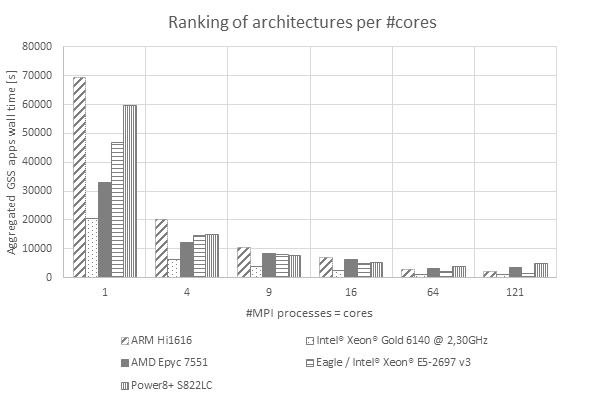
\includegraphics[width=1.\textwidth]{rank_archs_per_cores}
    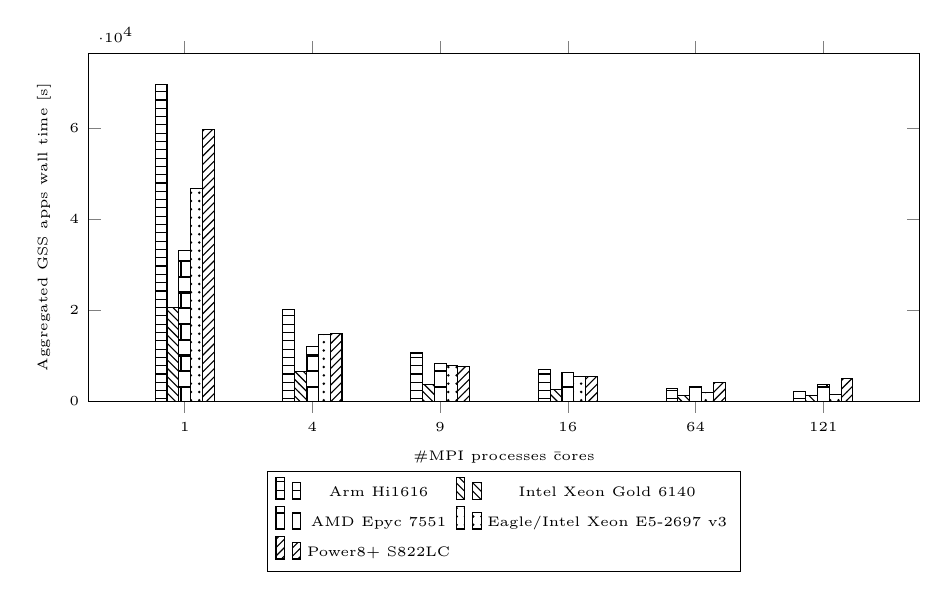
\begin{tikzpicture}
    \begin{axis}[
    	xtick={1,2,3,4,5,6},
    	xticklabels={1,4,9,16,64,121},
    	xlabel=\#MPI processes \= cores,
    	ylabel=Aggregated GSS apps wall time {[s]},
     	enlarge x limits=0.15,
     	ymin=0,
    	legend style={at={(0.5,-0.2)},
    	    anchor=north,legend columns=2},
      ybar=0pt,
      bar width=0.15cm, width=1.0\textwidth
    ]
    %Arm
    \addplot[black, pattern=horizontal lines]
    coordinates {(1,69475)(2,20195)(3,10571)(4,6877)(5,2750)(6,2165)};
    %Intel gold
    \addplot[black, pattern=north west lines]
    coordinates {(1,20624)(2,6428)(3,3616)(4,2526)(5,1140)(6,1249)};
    %AMD
    \addplot[black, pattern=bricks]
    coordinates {(1,33046)(2,12036)(3,8210)(4,6234)(5,3186)(6,3546)};
    %Eagle
    \addplot[black, pattern=dots]
    coordinates {(1,46790)(2,14646)(3,7874)(4,5393)(5,1934)(6,1487)};
    %Power8
    \addplot[black, pattern=north east lines]
    coordinates {(1,59679)(2,14838)(3,7669)(4,5318)(5,4015)(6,4995)};
    \legend{Arm Hi1616, Intel Xeon Gold 6140, AMD Epyc 7551, Eagle/Intel Xeon E5-2697 v3, Power8+ S822LC}
    \end{axis}
    \end{tikzpicture}
  \caption{Ranking of architectures across number of cores (processes)}\label{fig:rankarchspercore}
\end{subfigure}\hfill
\begin{subfigure}[t]{0.48\textwidth}
%%  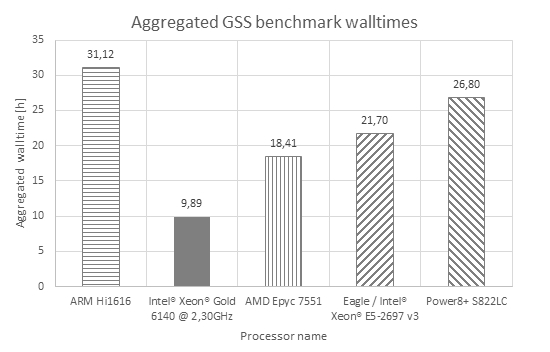
\includegraphics[width=1.\textwidth]{rank_archs_walltimes}
    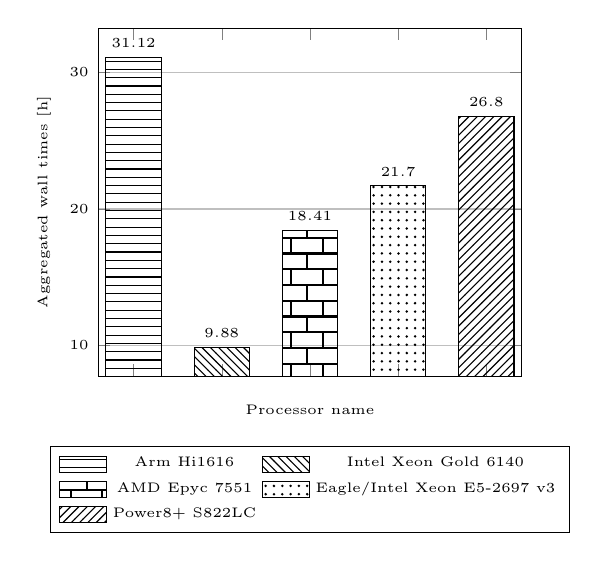
\begin{tikzpicture}
    \begin{groupplot}[
    legend columns=2,
    legend entries={Arm Hi1616, Intel Xeon Gold 6140, AMD Epyc 7551, Eagle/Intel Xeon E5-2697 v3, Power8+ S822LC},
    legend style={at={(0.5,-0.2)},
    	    anchor=north,legend columns=2},
    area legend,
    group style={
    xlabels at=edge bottom,
    ylabels at=edge left,
    xticklabels at=edge bottom},
    xtick = {1,2,3,4,5},
    ymajorgrids=true,
    nodes near coords,
    every node near coord/.append style={font=\tiny},
    xlabel={Processor name},
    ylabel={Aggregated wall times {[h]}},
    ]
    \nextgroupplot[bar width=20pt, xticklabel=\empty]
    \addplot[ybar, pattern=horizontal lines] coordinates {  (1, 31.12)};
    \addplot[ybar, pattern=north west lines] coordinates { (2, 9.88)};
    \addplot[ybar, pattern=bricks] coordinates {(3, 18.41)};
    \addplot[ybar, pattern=dots] coordinates {(4, 21.70)};
    \addplot[ybar, pattern=north east lines] coordinates {  (5, 26.8)};
    \end{groupplot}
    \end{tikzpicture}
  \caption{Aggregated GSS benchmark walltimes}
  \label{fig:rankarchswalltimes}
  \end{subfigure}
\begin{subfigure}[t]{0.48\textwidth}
%  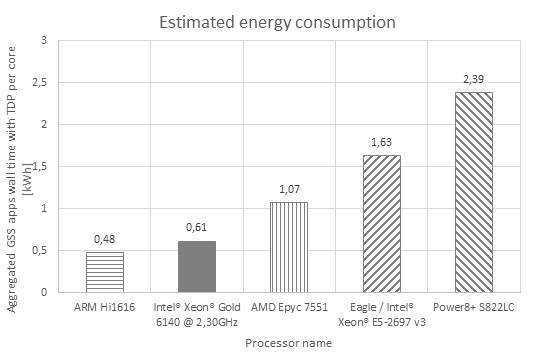
\includegraphics[width=1.\textwidth]{estimated_energy_consumption}
    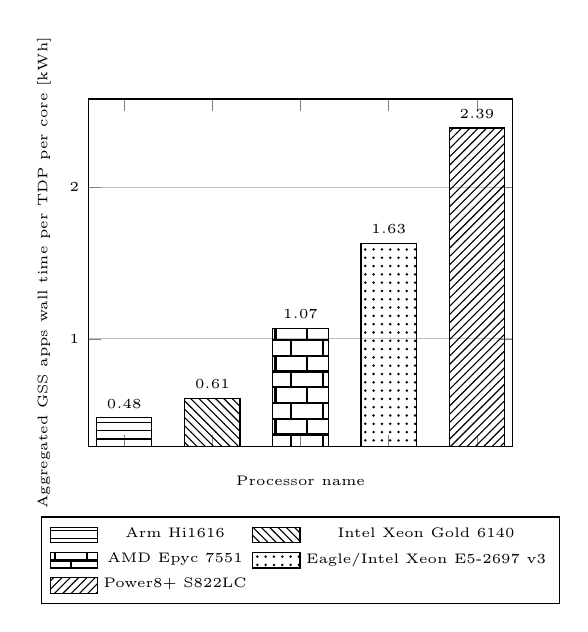
\begin{tikzpicture}
    \begin{groupplot}[
        legend columns=2,
        legend entries={Arm Hi1616, Intel Xeon Gold 6140, AMD Epyc 7551, Eagle/Intel Xeon E5-2697 v3, Power8+ S822LC},
        legend style={at={(0.5,-0.2)},
        	    anchor=north,legend columns=2},
        area legend,
        group style={
            xlabels at=edge bottom,
            ylabels at=edge left,
            xticklabels at=edge bottom},
        xtick = {1,2,3,4,5},
        ymajorgrids=true,
        nodes near coords,
        every node near coord/.append style={font=\tiny},
        xlabel={Processor name},
        ylabel={Aggregated GSS apps wall time per TDP per core {[kWh]}},
    ]
    \nextgroupplot[bar width=20pt, xticklabel=\empty]
    \addplot[ybar, pattern=horizontal lines] coordinates {  (1, 0.48)};
    \addplot[ybar, pattern=north west lines] coordinates { (2, 0.61)};
    \addplot[ybar, pattern=bricks] coordinates {(3, 1.07)};
    \addplot[ybar, pattern=dots] coordinates {(4, 1.63)};
    \addplot[ybar, pattern=north east lines] coordinates {  (5, 2.39)};
    \end{groupplot}
    \end{tikzpicture}
  \caption{Ranking of architectures based on estimated energy consumption (total power needed by CPU to finish all tests) - lower is better}
  \label{fig:estimatedenergyconsumption}
  \end{subfigure}\hfill
  %% 2 line
  \begin{subfigure}[t]{0.48\textwidth}
  \centering
%  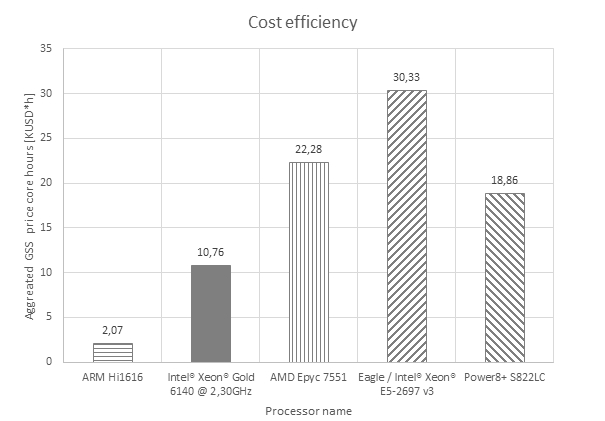
\includegraphics[width=1.\linewidth]{cost_efficiency}
    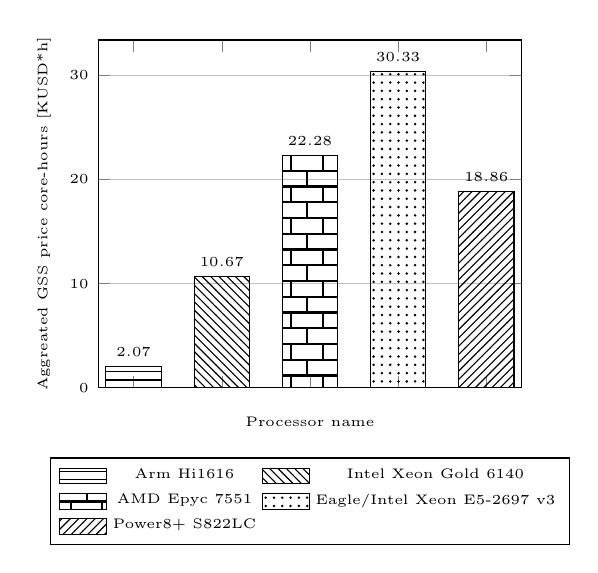
\begin{tikzpicture}
    \begin{groupplot}[
        legend columns=2,
        legend entries={Arm Hi1616, Intel Xeon Gold 6140, AMD Epyc 7551, Eagle/Intel Xeon E5-2697 v3, Power8+ S822LC},
        legend style={at={(0.5,-0.2)},
        	    anchor=north,legend columns=2},
        area legend,
        group style={
            xlabels at=edge bottom,
            ylabels at=edge left,
            xticklabels at=edge bottom},
        xtick = {1,2,3,4,5},
        ymin=0,
        ymajorgrids=true,
        nodes near coords,
        every node near coord/.append style={font=\tiny},
        xlabel={Processor name},
        ylabel={Aggreated GSS  price core-hours {[KUSD*h]}},
    ]
    \nextgroupplot[bar width=20pt, xticklabel=\empty]
    \addplot[ybar, pattern=horizontal lines] coordinates {  (1, 2.07)};
    \addplot[ybar, pattern=north west lines] coordinates { (2, 10.67)};
    \addplot[ybar, pattern=bricks] coordinates {(3, 22.28)};
    \addplot[ybar, pattern=dots] coordinates {(4, 30.33)};
    \addplot[ybar, pattern=north east lines] coordinates {  (5, 18.86)};
    \end{groupplot}
    \end{tikzpicture}    
  \caption{Ranking of architectures based on cost efficiency}
  \label{fig:costefficiency}
 \end{subfigure}%
 \bigbreak
 \caption{Benchmarking summary results}
\end{figure*}

In the scope of \textit{aggregated execution times} for the given number of cores it can be noted that in the whole range of the number of cores the winner is Intel\textregistered\ Xeon\textregistered\ Gold 6140 (Figure~\subref{fig:rankarchspercore}). Surprisingly, the AMD Epyc\textsuperscript{TM} is slower than the ARM Hi1616 when 64 or more cores are used and is also slower than the reference Intel\textregistered Xeon\textregistered\ E5-2697 when 9 or more cores are used.



By looking at the aggregated execution times across all tested applications, the winner turned out to be Intel\textregistered\ Xeon\textregistered\ Gold 6140 (Figure~\subref{fig:rankarchswalltimes}).



For the \textit{estimated cumulative energy consumption} (calculated as a sum of walltimes and TDP per used cores products expressed in kilowatt-hours) metric the winning processor is ARM Hi1616 representing the current tendency in HPC, where attention is turned to - generally speaking - energy efficient technologies. The second place winner is Intel\textregistered Xeon\textregistered\ Gold 6140 and Power8+ brings up the rear (Figure~\subref{fig:estimatedenergyconsumption}). 

The estimated power consumption chart is a good point of view when talking about green HPC computing. The presented results not exact, because they are dictated only by the estimated values based on the CPU's TDP. Nevertheless, assuming that almost all architectures use the same memory model - DDR4, it can be considered that most of the energy consumed is the energy utilized by the processor. In this scope, the best energy consumption ratio is characterized by the ARM architecture, which is absolutely designed for energy-saving solutions that is also widely used in mobile devices. The results for the new Intel Skylake architecture were a big surprise, which took the second place with a very similar result of about 20\% more. The AMD Epyc\textsuperscript{TM} presented a much worse result, but from our observations its internal architecture is better suited to applications in which I/O systems play an important role.

Another valuable finding is based on GSS cost efficiency analysis (Figure~\subref{fig:costefficiency}). ARM Hi1616 turned out to be approximately 9 times better than for Power8+ (with DDR3 and not utilized NVLinks) and 15 times better than the reference Intel\textregistered\ Xeon\textregistered\ E5-2697 processor, mostly due to its small number of expensive cores and relatively middling timing results.
Additionally, when talking about general processor characteristics extracted from all the tests performed, IBM Power8+ demonstrates particularly good performance for the applications with a big number of I/O such as Pandora, OpenSWPC, CMAQ/CCTM. The best results are obtained when the total output dominates over the input and RAM consumption. In many cases, it outperforms ARM Hi1616, Intel\textregistered\ Xeon\textregistered\ E5-2697, and AMD Epyc\textsuperscript{TM} for I/O intensive applications. On the other hand, Power8+ shows worse results than the above-mentioned processors if the applications are computationally extensive while producing a relatively small amount of output. This is the case of the IPF and ABMS applications. On all processors, all benchmarks show the highest efficiency if the number of MPI processes is between 2 and the total number of physical cores. After that, the efficiency usually drops remarkably as hyper threading is not utilised properly. At the same time, quite often the highest speedup is reached when the number of MPI processes is significantly more than 20. It would be interesting to perform the tests on the testbeds including more nodes. 



When analysed simultaneously, all the above results prove that the most promising ARM processor in the context of cost and energy consumption is the slowest at the same time (mostly due to low clock frequency). Other competitor, Intel\textregistered\ Xeon\textregistered\ Gold 6140, is 5 times less cost efficient for GSS benchmark and slightly worse in the energy consumption but it is approximately 3 times quicker regarding the aggregated execution time. In other words, the future HPC investors having the above information in place have the ability to decide which direction to follow: reach high compute intensity, minimize costs, or try to find the golden mean.

Table~\ref{tab:ranking} presents the summarised results for each individual architecture in three separate domains: walltime, energy efficiency and cost efficiency. The numbers reflects the weighted points referring to the overall applications results in a given category (in this case the less is better). In general, the most promising processor is Intel\textregistered\ Xeon\textregistered\ Gold 6140 but those individuals for whom costs and environmental aspects are the most important should look closely at ARM Hi1616.
    
    
\begin{table}
\caption{Ranking of all tested architectures (\textit{less is better})}
\label{tab:ranking}
\centering
\begin{tabular}{l|c|c|c|}
\cline{2-4}
 & \textbf{Walltime} & \textbf{\begin{tabular}[c]{@{}c@{}}Energy\\ efficiency\end{tabular}} & \textbf{\begin{tabular}[c]{@{}c@{}}Cost\\ efficiency\end{tabular}} \\ \hline
\multicolumn{1}{|l|}{\textbf{ARM Hi1616}} & 1.0 & 0.2 & 0.1 \\ \hline
\multicolumn{1}{|l|}{\textbf{Intel\textregistered\ Xeon\textregistered\ Gold 6140}} & 0.3 & 0.3 & 0.4 \\ \hline
\multicolumn{1}{|l|}{\textbf{AMD Epyc\textsuperscript{TM} 7551}} & 0.6 & 0.4 & 0.7 \\ \hline
\multicolumn{1}{|l|}{\textbf{Intel\textregistered\ Xeon\textregistered\ E5-2697}} & 0.7 & 0.7 & 1.0 \\ \hline
\multicolumn{1}{|l|}{\textbf{Power8+ S822LC}} & 0.9 & 1.0 & 0.6 \\ \hline
\end{tabular}
\end{table}

 In general, it can be said, the most promising processor is Intel\textregistered\ Xeon\textregistered\ Gold 6140 but those individuals for whom costs and environmental aspects are the most important should look closely at ARM Hi1616.



\section{Future work}
The proposed benchmark gives a good evaluation tool for a relatively automatic way of proceeding with tests and receiving results which will directly allow using the best HPC architecture.  It means that finally the end user or the resource owner may have different criteria to fulfil their requirements. The resource owner will focus on parameters which are efficient globally (all applications running on the machine), cost efficiency (TCO shown as CAPEX and OPEX, i.e. the investment costs vs. maintenance costs of the HPC). The end user will, however, concentrate on the fastest way to receive results and the most efficient way of parallelisation.

From that point of view the benchmark could be extended by testing automatically
the scalability of the e-Infrastructure and the energy consumption of the running benchmark. A final step of the benchmark could interpret the results for both groups of users and propose the best HPC system in terms of size and architecture (CPU, memory size, aggregated speed to external memory, if necessary).


\section*{Acknowledgements}
This work has been supported by the CoeGSS (Centre of Excellence for Global System Science) project and has been partly funded by the European Commission's ICT activity of the H2020 Programme under grant agreement number: 676547.

\openaccess

\bibliography{example}
\end{document}
